\documentclass[a4paper,14pt,oneside,openany]{memoir}

%%%%%%%%%%%%%%%%%%%%%%%%%%%%%%%%%%%%%%%%%%%%%%%%%%%%%%%%%%%%%%%%%%%%%%%%%%%%%%%%
%%%% Файл упрощённых настроек шаблона, общих для диссертации и автореферата %%%%
%%%%%%%%%%%%%%%%%%%%%%%%%%%%%%%%%%%%%%%%%%%%%%%%%%%%%%%%%%%%%%%%%%%%%%%%%%%%%%%%

%%% Режим черновика %%%
\makeatletter
\@ifundefined{c@draft}{
  \newcounter{draft}
  \setcounter{draft}{0}  % 0 --- чистовик (максимальное соблюдение ГОСТ)
                         % 1 --- черновик (отклонения от ГОСТ, но быстрая
                         %       сборка итоговых PDF)
}{}
\makeatother

%%% Пометки в тексте %%%
\makeatletter
\@ifundefined{c@showmarkup}{
  \newcounter{showmarkup}
  \setcounter{showmarkup}{0}  % 0 --- скрыть пометки
                              % 1 --- показывать пометки
}{}
\makeatother

%%% Использование в pdflatex шрифтов не по-умолчанию %%%
\makeatletter
\@ifundefined{c@usealtfont}{
  \newcounter{usealtfont}
  \setcounter{usealtfont}{1}    % 0 --- шрифты на базе Computer Modern
                                % 1 --- использовать пакет pscyr, при его
                                %       наличии
                                % 2 --- использовать пакет XCharter, при наличии
                                %       подходящей версии
}{}
\makeatother

%%% Использование в xelatex и lualatex семейств шрифтов %%%
\makeatletter
\@ifundefined{c@fontfamily}{
  \newcounter{fontfamily}
  \setcounter{fontfamily}{1}  % 0 --- CMU семейство. Используется как fallback;
                              % 1 --- Шрифты от MS (Times New Roman и компания)
                              % 2 --- Семейство Liberation
}{}
\makeatother


%%% Вывод типов ссылок в библиографии %%%
\makeatletter
\@ifundefined{c@mediadisplay}{
  \newcounter{mediadisplay}
  \setcounter{mediadisplay}{1}   % 0 --- не делать ничего; надписи [Текст] и
                                 %       [Эл. ресурс] будут выводиться только в ссылках с
                                 %       заполненным полем `media`;
                                 % 1 --- автоматически добавлять надпись [Текст] к ссылкам с
                                 %       незаполненным полем `media`; таким образом, у всех
                                 %       источников будет указан тип, что соответствует
                                 %       требованиям ГОСТ
                                 % 2 --- автоматически удалять надписи [Текст], [Эл. Ресурс] и др.;
                                 %       не соответствует ГОСТ
                                 % 3 --- автоматически удалять надпись [Текст];
                                 %       не соответствует ГОСТ
                                 % 4 --- автоматически удалять надпись [Эл. Ресурс];
                                 %       не соответствует ГОСТ
}{}
\makeatother

%%% Предкомпиляция tikz рисунков для ускорения работы %%%
\makeatletter
\@ifundefined{c@imgprecompile}{
  \newcounter{imgprecompile}
  \setcounter{imgprecompile}{0}   % 0 --- без предкомпиляции;
                                  % 1 --- пользоваться предварительно
                                  %       скомпилированными pdf вместо генерации
                                  %       заново из tikz
}{}
\makeatother
            % общие настройки шаблона
%%% Проверка используемого TeX-движка %%%
\newif\ifxetexorluatex   % определяем новый условный оператор (http://tex.stackexchange.com/a/47579)
\ifxetex
    \xetexorluatextrue
\else
    \ifluatex
        \xetexorluatextrue
    \else
        \xetexorluatexfalse
    \fi
\fi

\usepackage{etoolbox}[2015/08/02]   % Для продвинутой проверки разных условий
\providebool{presentation}

\usepackage{comment}    % Позволяет убирать блоки текста (добавляет
                        % окружение comment и команду \excludecomment)

%%% Поля и разметка страницы %%%
\usepackage{pdflscape}  % Для включения альбомных страниц
\usepackage{geometry}   % Для последующего задания полей

%%% Математические пакеты %%%
\usepackage{amsthm,amsmath,amscd}   % Математические дополнения от AMS
\usepackage{amsfonts,amssymb}       % Математические дополнения от AMS
\usepackage{mathtools}              % Добавляет окружение multlined
\usepackage{xfrac}                  % Красивые дроби
\usepackage[
    locale = DE,
    list-separator       = {;\,},
    list-final-separator = {;\,},
    list-pair-separator  = {;\,},
    list-units           = single,
    range-units          = single,
    range-phrase={\text{\ensuremath{-}}},
    % quotient-mode        = fraction, % красивые дроби могут не соответствовать ГОСТ
    fraction-function    = \sfrac,
    separate-uncertainty,
    ]{siunitx}[=v2]                 % Размерности SI
\sisetup{inter-unit-product = \ensuremath{{}\cdot{}}}

% Кириллица в нумерации subequations
% Для правильной работы требуется выполнение сразу после загрузки пакетов
\patchcmd{\subequations}{\def\theequation{\theparentequation\alph{equation}}}
{\def\theequation{\theparentequation\asbuk{equation}}}
{\typeout{subequations patched}}{\typeout{subequations not patched}}

%%%% Установки для размера шрифта 14 pt %%%%
%% Формирование переменных и констант для сравнения (один раз для всех подключаемых файлов)%%
%% должно располагаться до вызова пакета fontspec или polyglossia, потому что они сбивают его работу
\newlength{\curtextsize}
\newlength{\bigtextsize}
\setlength{\bigtextsize}{13.9pt}

\makeatletter
%\show\f@size    % неплохо для отслеживания, но вызывает стопорение процесса,
                 % если документ компилируется без команды  -interaction=nonstopmode
\setlength{\curtextsize}{\f@size pt}
\makeatother

%%% Кодировки и шрифты %%%
\ifxetexorluatex
    \ifpresentation
        \providecommand*\autodot{} % quick fix for polyglossia 1.50
    \fi
    \PassOptionsToPackage{no-math}{fontspec}    % https://tex.stackexchange.com/a/26295/104425
    \usepackage{polyglossia}[2014/05/21]        % Поддержка многоязычности
                                        % (fontspec подгружается автоматически)
\else
   %%% Решение проблемы копирования текста в буфер кракозябрами
    \ifnumequal{\value{usealtfont}}{0}{}{
        \input glyphtounicode.tex
        \input glyphtounicode-cmr.tex %from pdfx package
        \pdfgentounicode=1
    }
    \usepackage{cmap}   % Улучшенный поиск русских слов в полученном pdf-файле
    \ifnumequal{\value{usealtfont}}{2}{}{
        \defaulthyphenchar=127  % Если стоит до fontenc, то переносы
                                % не впишутся в выделяемый текст при
                                % копировании его в буфер обмена
    }
    \usepackage{textcomp}
    \usepackage[T1,T2A]{fontenc}                    % Поддержка русских букв
    \ifnumequal{\value{usealtfont}}{1}{% Используется pscyr, при наличии
        \IfFileExists{pscyr.sty}{\usepackage{pscyr}}{}  % Подключение pscyr
    }{}
    \usepackage[utf8]{inputenc}[2014/04/30]         % Кодировка utf8
    \usepackage[english, russian]{babel}[2014/03/24]% Языки: русский, английский
    \makeatletter\AtBeginDocument{\let\@elt\relax}\makeatother % babel 3.40 fix
    \ifnumequal{\value{usealtfont}}{2}{
        % http://dxdy.ru/post1238763.html#p1238763
        \usepackage[scaled=0.914]{XCharter}[2017/12/19] % Подключение русифицированных шрифтов XCharter
        \usepackage[charter, vvarbb, scaled=1.048]{newtxmath}[2017/12/14]
        \ifpresentation
        \else
            \setDisplayskipStretch{-0.078}
        \fi
    }{}
\fi

%%% Оформление абзацев %%%
\ifpresentation
\else
    \indentafterchapter     % Красная строка после заголовков типа chapter
    \usepackage{indentfirst}
\fi

%%% Цвета %%%
\ifpresentation
\else
    \usepackage[dvipsnames, table, hyperref]{xcolor} % Совместимо с tikz
\fi

%%% Таблицы %%%
\usepackage{longtable,ltcaption} % Длинные таблицы
\usepackage{multirow,makecell}   % Улучшенное форматирование таблиц
\usepackage{tabu, tabulary}      % таблицы с автоматически подбирающейся
                                 % шириной столбцов (tabu обязательно
                                 % до hyperref вызывать)
\makeatletter
%https://github.com/tabu-issues-for-future-maintainer/tabu/issues/26
\@ifpackagelater{longtable}{2020/02/07}{
\def\tabuendlongtrial{%
    \LT@echunk  \global\setbox\LT@gbox \hbox{\unhbox\LT@gbox}\kern\wd\LT@gbox
                \LT@get@widths
}%
}{}
\makeatother

\usepackage{threeparttable}      % автоматический подгон ширины подписи таблицы

%%% Общее форматирование
\usepackage{soulutf8}% Поддержка переносоустойчивых подчёркиваний и зачёркиваний
\usepackage{icomma}  % Запятая в десятичных дробях

%%% Оптимизация расстановки переносов и длины последней строки абзаца
\IfFileExists{impnattypo.sty}{% проверка установленности пакета impnattypo
    \ifluatex
        \ifnumequal{\value{draft}}{1}{% Черновик
            \usepackage[hyphenation, lastparline, nosingleletter, homeoarchy,
            rivers, draft]{impnattypo}
        }{% Чистовик
            \usepackage[hyphenation, lastparline, nosingleletter]{impnattypo}
        }
    \else
        \usepackage[hyphenation, lastparline]{impnattypo}
    \fi
}{}

%% Векторная графика

\usepackage{tikz}                   % Продвинутый пакет векторной графики
\usetikzlibrary{chains}             % Для примера tikz рисунка
\usetikzlibrary{shapes.geometric}   % Для примера tikz рисунка
\usetikzlibrary{shapes.symbols}     % Для примера tikz рисунка
\usetikzlibrary{arrows}             % Для примера tikz рисунка
\usetikzlibrary{positioning}
\usetikzlibrary{snakes,arrows,shapes}
\usepackage{amsmath}
%

%%% Гиперссылки %%%
\ifxetexorluatex
    \let\CYRDZE\relax
\fi
\usepackage{hyperref}[2012/11/06]

%%% Изображения %%%
\usepackage{graphicx}[2014/04/25]   % Подключаем пакет работы с графикой
\usepackage{caption}                % Подписи рисунков и таблиц
\usepackage{subcaption}             % Подписи подрисунков и подтаблиц
\usepackage{pdfpages}               % Добавление внешних pdf файлов

%%% Счётчики %%%
\usepackage{aliascnt}
\usepackage[figure,table]{totalcount}   % Счётчик рисунков и таблиц
\usepackage{totcount}   % Пакет создания счётчиков на основе последнего номера
                        % подсчитываемого элемента (может требовать дважды
                        % компилировать документ)
\usepackage{totpages}   % Счётчик страниц, совместимый с hyperref (ссылается
                        % на номер последней страницы). Желательно ставить
                        % последним пакетом в преамбуле

%%% Продвинутое управление групповыми ссылками (пока только формулами) %%%
\ifpresentation
\else
    \usepackage[russian]{cleveref} % cleveref имеет сложности со считыванием
    % языка из babel. Такое решение русификации вывода выбрано вместо
    % определения в documentclass из опасности что-то лишнее передать во все
    % остальные пакеты, включая библиографию.

    % Добавление возможности использования пробелов в \labelcref
    % https://tex.stackexchange.com/a/340502/104425
    \usepackage{kvsetkeys}
    \makeatletter
    \let\org@@cref\@cref
    \renewcommand*{\@cref}[2]{%
        \edef\process@me{%
            \noexpand\org@@cref{#1}{\zap@space#2 \@empty}%
        }\process@me
    }
    \makeatother
\fi

\usepackage{placeins} % для \FloatBarrier

\ifnumequal{\value{draft}}{1}{% Черновик
    \usepackage[firstpage]{draftwatermark}
    \SetWatermarkText{DRAFT}
    \SetWatermarkFontSize{14pt}
    \SetWatermarkScale{15}
    \SetWatermarkAngle{45}
}{}

%%% Цитата, не приводимая в автореферате:
% возможно, актуальна только для biblatex
%\newcommand{\citeinsynopsis}[1]{\ifsynopsis\else ~\cite{#1} \fi}

% если текущий процесс запущен библиотекой tikz-external, то прекомпиляция должна быть включена
\ifdefined\tikzexternalrealjob
    \setcounter{imgprecompile}{1}
\fi

\ifnumequal{\value{imgprecompile}}{1}{% Только если у нас включена предкомпиляция
    \usetikzlibrary{external}   % подключение возможности предкомпиляции
    \tikzexternalize[prefix=images/cache/,optimize command away=\includepdf] % activate! % здесь можно указать отдельную папку для скомпилированных файлов
    \ifxetex
        \tikzset{external/up to date check={diff}}
    \fi
}{}




%%% Прикладные пакеты %%%
%\usepackage{calc}               % Пакет для расчётов параметров, например длины

%%% Для добавления Стр. над номерами страниц в оглавлении
%%% http://tex.stackexchange.com/a/306950
\usepackage{afterpage}

%%% Списки %%%
\usepackage{enumitem}

%%% Оформление списка обозначений
\usepackage[intoc]{nomencl}
\makenomenclature
\setlength{\nomitemsep}{-.8\parsep}





\usepackage{fr-longtable}    %ради \endlasthead

% Листинги с исходным кодом программ
\usepackage{fancyvrb}
\usepackage{listings}
\lccode`\~=0\relax %Без этого хака из-за особенностей пакета listings перестают работать конструкции с \MakeLowercase и т. п. в (xe|lua)latex

% Русская традиция начертания греческих букв
\usepackage{upgreek} % прямые греческие ради русской традиции

%%% Микротипографика
%\ifnumequal{\value{draft}}{0}{% Только если у нас режим чистовика
	%    \usepackage[final, babel, shrink=45]{microtype}[2016/05/14] % улучшает представление букв и слов в строках, может помочь при наличии отдельно висящих слов
	%}{}

% Отметка о версии черновика на каждой странице
% Чтобы работало надо в своей локальной копии по инструкции
% https://www.ctan.org/pkg/gitinfo2 создать небходимые файлы в папке
% ./git/hooks
% If you’re familiar with tweaking git, you can probably work it out for
% yourself. If not, I suggest you follow these steps:
% 1. First, you need a git repository and working tree. For this example,
% let’s suppose that the root of the working tree is in ~/compsci
% 2. Copy the file post-xxx-sample.txt (which is in the same folder of
% your TEX distribution as this pdf) into the git hooks directory in your
% working copy. In our example case, you should end up with a file called
% ~/compsci/.git/hooks/post-checkout
% 3. If you’re using a unix-like system, don’t forget to make the file executable.
% Just how you do this is outside the scope of this manual, but one
% possible way is with commands such as this:
% chmod g+x post-checkout.
% 4. Test your setup with “git checkout master” (or another suitable branch
% name). This should generate copies of gitHeadInfo.gin in the directories
% you intended.
% 5. Now make two more copies of this file in the same directory (hooks),
% calling them post-commit and post-merge, and you’re done. As before,
% users of unix-like systems should ensure these files are marked as
% executable.
\ifnumequal{\value{draft}}{1}{% Черновик
	\IfFileExists{.git/gitHeadInfo.gin}{
		\usepackage[mark,pcount]{gitinfo2}
		\renewcommand{\gitMark}{rev.\gitAbbrevHash\quad\gitCommitterEmail\quad\gitAuthorIsoDate}
		\renewcommand{\gitMarkFormat}{\rmfamily\color{Gray}\small\bfseries}
	}{}
}{}         % Пакеты общие для диссертации и автореферата
%%% Прикладные пакеты %%%
%\usepackage{calc}               % Пакет для расчётов параметров, например длины

%%% Для добавления Стр. над номерами страниц в оглавлении
%%% http://tex.stackexchange.com/a/306950
\usepackage{afterpage}

%%% Списки %%%
\usepackage{enumitem}

%%% Оформление списка обозначений
\usepackage[intoc]{nomencl}
\makenomenclature
\setlength{\nomitemsep}{-.8\parsep}
    % Пакеты для диссертации
\usepackage{fr-longtable}    %ради \endlasthead

% Листинги с исходным кодом программ
\usepackage{fancyvrb}
\usepackage{listings}
\lccode`\~=0\relax %Без этого хака из-за особенностей пакета listings перестают работать конструкции с \MakeLowercase и т. п. в (xe|lua)latex

% Русская традиция начертания греческих букв
\usepackage{upgreek} % прямые греческие ради русской традиции

%%% Микротипографика
%\ifnumequal{\value{draft}}{0}{% Только если у нас режим чистовика
%    \usepackage[final, babel, shrink=45]{microtype}[2016/05/14] % улучшает представление букв и слов в строках, может помочь при наличии отдельно висящих слов
%}{}

% Отметка о версии черновика на каждой странице
% Чтобы работало надо в своей локальной копии по инструкции
% https://www.ctan.org/pkg/gitinfo2 создать небходимые файлы в папке
% ./git/hooks
% If you’re familiar with tweaking git, you can probably work it out for
% yourself. If not, I suggest you follow these steps:
% 1. First, you need a git repository and working tree. For this example,
% let’s suppose that the root of the working tree is in ~/compsci
% 2. Copy the file post-xxx-sample.txt (which is in the same folder of
% your TEX distribution as this pdf) into the git hooks directory in your
% working copy. In our example case, you should end up with a file called
% ~/compsci/.git/hooks/post-checkout
% 3. If you’re using a unix-like system, don’t forget to make the file executable.
% Just how you do this is outside the scope of this manual, but one
% possible way is with commands such as this:
% chmod g+x post-checkout.
% 4. Test your setup with “git checkout master” (or another suitable branch
% name). This should generate copies of gitHeadInfo.gin in the directories
% you intended.
% 5. Now make two more copies of this file in the same directory (hooks),
% calling them post-commit and post-merge, and you’re done. As before,
% users of unix-like systems should ensure these files are marked as
% executable.
\ifnumequal{\value{draft}}{1}{% Черновик
   \IfFileExists{.git/gitHeadInfo.gin}{
      \usepackage[mark,pcount]{gitinfo2}
      \renewcommand{\gitMark}{rev.\gitAbbrevHash\quad\gitCommitterEmail\quad\gitAuthorIsoDate}
      \renewcommand{\gitMarkFormat}{\rmfamily\color{Gray}\small\bfseries}
   }{}
}{}   % Пакеты для специфических пользовательских задач

%%%%%%%%%%%%%%%%%%%%%%%%%%%%%%%%%%%%%%%%%%%%%%%%%%%%%%
%%%% Файл упрощённых настроек шаблона диссертации %%%%
%%%%%%%%%%%%%%%%%%%%%%%%%%%%%%%%%%%%%%%%%%%%%%%%%%%%%%

%%% Инициализирование переменных, не трогать!  %%%
\newcounter{intvl}
\newcounter{otstup}
\newcounter{contnumeq}
\newcounter{contnumfig}
\newcounter{contnumtab}
\newcounter{pgnum}
\newcounter{chapstyle}
\newcounter{headingdelim}
\newcounter{headingalign}
\newcounter{headingsize}
%%%%%%%%%%%%%%%%%%%%%%%%%%%%%%%%%%%%%%%%%%%%%%%%%%%%%%

%%% Область упрощённого управления оформлением %%%

%% Интервал между заголовками и между заголовком и текстом %%
% Заголовки отделяют от текста сверху и снизу
% тремя интервалами (ГОСТ Р 7.0.11-2011, 5.3.5)
\setcounter{intvl}{3}               % Коэффициент кратности к размеру шрифта

%% Отступы у заголовков в тексте %%
\setcounter{otstup}{0}              % 0 --- без отступа; 1 --- абзацный отступ

%% Нумерация формул, таблиц и рисунков %%
% Нумерация формул
\setcounter{contnumeq}{0}   % 0 --- пораздельно (во введении подряд,
                            %       без номера раздела);
                            % 1 --- сквозная нумерация по всей диссертации
% Нумерация рисунков
\setcounter{contnumfig}{0}  % 0 --- пораздельно (во введении подряд,
                            %       без номера раздела);
                            % 1 --- сквозная нумерация по всей диссертации
% Нумерация таблиц
\setcounter{contnumtab}{1}  % 0 --- пораздельно (во введении подряд,
                            %       без номера раздела);
                            % 1 --- сквозная нумерация по всей диссертации

%% Оглавление %%
\setcounter{pgnum}{1}       % 0 --- номера страниц никак не обозначены;
                            % 1 --- Стр. над номерами страниц (дважды
                            %       компилировать после изменения настройки)
\settocdepth{subsection}    % до какого уровня подразделов выносить в оглавление
\setsecnumdepth{subsection} % до какого уровня нумеровать подразделы


%% Текст и форматирование заголовков %%
\setcounter{chapstyle}{1}     % 0 --- разделы только под номером;
                              % 1 --- разделы с названием "Глава" перед номером
\setcounter{headingdelim}{1}  % 0 --- номер отделен пропуском в 1em или \quad;
                              % 1 --- номера разделов и приложений отделены
                              %       точкой с пробелом, подразделы пропуском
                              %       без точки;
                              % 2 --- номера разделов, подразделов и приложений
                              %       отделены точкой с пробелом.

%% Выравнивание заголовков в тексте %%
\setcounter{headingalign}{0}  % 0 --- по центру;
                              % 1 --- по левому краю

%% Размеры заголовков в тексте %%
\setcounter{headingsize}{0}   % 0 --- по ГОСТ, все всегда 14 пт;
                              % 1 --- пропорционально изменяющийся размер
                              %       в зависимости от базового шрифта

%% Подпись таблиц %%

% Смещение строк подписи после первой строки
\newcommand{\tabindent}{0cm}

% Тип форматирования заголовка таблицы:
% plain --- название и текст в одной строке
% split --- название и текст в разных строках
\newcommand{\tabformat}{plain}

%%% Настройки форматирования таблицы `plain`

% Выравнивание по центру подписи, состоящей из одной строки:
% true  --- выравнивать
% false --- не выравнивать
\newcommand{\tabsinglecenter}{false}

% Выравнивание подписи таблиц:
% justified   --- выравнивать как обычный текст («по ширине»)
% centering   --- выравнивать по центру
% centerlast  --- выравнивать по центру только последнюю строку
% centerfirst --- выравнивать по центру только первую строку (не рекомендуется)
% raggedleft  --- выравнивать по правому краю
% raggedright --- выравнивать по левому краю
\newcommand{\tabjust}{justified}

% Разделитель записи «Таблица #» и названия таблицы
\newcommand{\tablabelsep}{~\cyrdash\ }

%%% Настройки форматирования таблицы `split`

% Положение названия таблицы:
% \centering   --- выравнивать по центру
% \raggedleft  --- выравнивать по правому краю
% \raggedright --- выравнивать по левому краю
\newcommand{\splitformatlabel}{\raggedleft}

% Положение текста подписи:
% \centering   --- выравнивать по центру
% \raggedleft  --- выравнивать по правому краю
% \raggedright --- выравнивать по левому краю
\newcommand{\splitformattext}{\raggedright}

%% Подпись рисунков %%
%Разделитель записи «Рисунок #» и названия рисунка
\newcommand{\figlabelsep}{~\cyrdash\ }  % (ГОСТ 2.105, 4.3.1)
                                        % "--- здесь не работает

%%% Цвета гиперссылок %%%
% Latex color definitions: http://latexcolor.com/
\definecolor{linkcolor}{rgb}{0.9,0,0}
\definecolor{citecolor}{rgb}{0,0.6,0}
\definecolor{urlcolor}{rgb}{0,0,1}
%\definecolor{linkcolor}{rgb}{0,0,0} %black
%\definecolor{citecolor}{rgb}{0,0,0} %black
%\definecolor{urlcolor}{rgb}{0,0,0} %black
      % Упрощённые настройки шаблона
\newcommand{\statementOneRU}{
    Ваше первое положение на русском.
}
\newcommand{\statementOneEN}{
    Your first statement in English.
}


\newcommand{\statementTwoRU}{
    Ваше второе положение на русском.
}
\newcommand{\statementTwoEN}{
    Your second statement in English.
} % тут ваши положения 

% Новые переменные, которые могут использоваться во всём проекте
% ГОСТ 7.0.11-2011
% 9.2 Оформление текста автореферата диссертации
% 9.2.1 Общая характеристика работы включает в себя следующие основные структурные
% элементы:
% актуальность темы исследования;
\newcommand{\actualityTXT}{Актуальность темы.}
% степень ее разработанности;
\newcommand{\progressTXT}{Степень разработанности темы.}
% цели и задачи;
\newcommand{\aimTXT}{Целью}
\newcommand{\tasksTXT}{задачи}
% научную новизну;
\newcommand{\noveltyTXT}{Научная новизна:}
% теоретическую и практическую значимость работы;
%\newcommand{\influenceTXT}{Теоретическая и практическая значимость}
% или чаще используют просто
\newcommand{\influenceTXT}{Практическая значимость}
% методологию и методы исследования;
\newcommand{\methodsTXT}{Методология и методы исследования.}
% положения, выносимые на защиту;
\newcommand{\defpositionsTXT}{Основные положения, выносимые на~защиту:}
% степень достоверности и апробацию результатов.
\newcommand{\reliabilityTXT}{Достоверность}
\newcommand{\probationTXT}{Апробация работы.}

\newcommand{\contributionTXT}{Личный вклад.}
\newcommand{\publicationsTXT}{Публикации.}


%%% Заголовки библиографии:

% для автореферата:
\newcommand{\bibtitleauthor}{Публикации автора по теме диссертации}

% для стиля библиографии `\insertbiblioauthorgrouped`
\newcommand{\bibtitleauthorvak}{В изданиях из списка ВАК РФ}
\newcommand{\bibtitleauthorscopus}{В изданиях, входящих в международную базу цитирования Scopus}
\newcommand{\bibtitleauthorwos}{В изданиях, входящих в международную базу цитирования Web of Science}
\newcommand{\bibtitleauthorother}{В прочих изданиях}
\newcommand{\bibtitleauthorconf}{В сборниках трудов конференций}
\newcommand{\bibtitleauthorpatent}{Зарегистрированные патенты}
\newcommand{\bibtitleauthorprogram}{Зарегистрированные программы для ЭВМ}

% для стиля библиографии `\insertbiblioauthorimportant`:
\newcommand{\bibtitleauthorimportant}{Наиболее значимые \protect\MakeLowercase\bibtitleauthor}

% для списка литературы в диссертации и списка чужих работ в автореферате:
\newcommand{\bibtitlefull}{Список литературы} % (ГОСТ Р 7.0.11-2011, 4)
         % Новые переменные, для всего проекта

%%% Кодировки и шрифты %%%
\ifxetexorluatex
    % Язык по-умолчанию русский с поддержкой приятных команд пакета babel
    \setmainlanguage[babelshorthands=true]{russian}
    % Дополнительный язык = английский (в американской вариации по-умолчанию)
    \setotherlanguage{english}

    % Проверка существования шрифтов. Недоступна в pdflatex
    \ifnumequal{\value{fontfamily}}{1}{
        \IfFontExistsTF{Times New Roman}{}{\setcounter{fontfamily}{0}}
    }{}
    \ifnumequal{\value{fontfamily}}{2}{
        \IfFontExistsTF{LiberationSerif}{}{\setcounter{fontfamily}{0}}
    }{}

    \ifnumequal{\value{fontfamily}}{0}{                    % Семейство шрифтов CMU. Используется как fallback
        \setmonofont{CMU Typewriter Text}                  % моноширинный шрифт
        \newfontfamily\cyrillicfonttt{CMU Typewriter Text} % моноширинный шрифт для кириллицы
        \defaultfontfeatures{Ligatures=TeX}                % стандартные лигатуры TeX, замены нескольких дефисов на тире и т. п. Настройки моноширинного шрифта должны идти до этой строки, чтобы при врезках кода программ в коде не применялись лигатуры и замены дефисов
        \setmainfont{CMU Serif}                            % Шрифт с засечками
        \newfontfamily\cyrillicfont{CMU Serif}             % Шрифт с засечками для кириллицы
        \setsansfont{CMU Sans Serif}                       % Шрифт без засечек
        \newfontfamily\cyrillicfontsf{CMU Sans Serif}      % Шрифт без засечек для кириллицы
    }

    \ifnumequal{\value{fontfamily}}{1}{                    % Семейство MS шрифтов
        \setmonofont{Courier New}                          % моноширинный шрифт
        \newfontfamily\cyrillicfonttt{Courier New}         % моноширинный шрифт для кириллицы
        \defaultfontfeatures{Ligatures=TeX}                % стандартные лигатуры TeX, замены нескольких дефисов на тире и т. п. Настройки моноширинного шрифта должны идти до этой строки, чтобы при врезках кода программ в коде не применялись лигатуры и замены дефисов
        \setmainfont{Times New Roman}                      % Шрифт с засечками
        \newfontfamily\cyrillicfont{Times New Roman}       % Шрифт с засечками для кириллицы
        \setsansfont{Arial}                                % Шрифт без засечек
        \newfontfamily\cyrillicfontsf{Arial}               % Шрифт без засечек для кириллицы
    }

    \ifnumequal{\value{fontfamily}}{2}{                    % Семейство шрифтов Liberation (https://pagure.io/liberation-fonts)
        \setmonofont{LiberationMono}[Scale=0.87] % моноширинный шрифт
        \newfontfamily\cyrillicfonttt{LiberationMono}[     % моноширинный шрифт для кириллицы
            Scale=0.87]
        \defaultfontfeatures{Ligatures=TeX}                % стандартные лигатуры TeX, замены нескольких дефисов на тире и т. п. Настройки моноширинного шрифта должны идти до этой строки, чтобы при врезках кода программ в коде не применялись лигатуры и замены дефисов
        \setmainfont{LiberationSerif}                      % Шрифт с засечками
        \newfontfamily\cyrillicfont{LiberationSerif}       % Шрифт с засечками для кириллицы
        \setsansfont{LiberationSans}                       % Шрифт без засечек
        \newfontfamily\cyrillicfontsf{LiberationSans}      % Шрифт без засечек для кириллицы
    }

\else
    \ifnumequal{\value{usealtfont}}{1}{% Используется pscyr, при наличии
        \IfFileExists{pscyr.sty}{\renewcommand{\rmdefault}{ftm}}{}
    }{}
\fi
            % Определение шрифтов (частичное)
%%% Шаблон %%%
\DeclareRobustCommand{\fixme}{\textcolor{red}}  % решаем проблему превращения
                                % названия цвета в результате \MakeUppercase,
                                % http://tex.stackexchange.com/a/187930,
                                % \DeclareRobustCommand protects \fixme
                                % from expanding inside \MakeUppercase
\AtBeginDocument{%
    \setlength{\parindent}{2.5em}                   % Абзацный отступ. Должен быть одинаковым по всему тексту и равен пяти знакам (ГОСТ Р 7.0.11-2011, 5.3.7).
}

%%% Таблицы %%%
\DeclareCaptionLabelSeparator{tabsep}{\tablabelsep} % нумерация таблиц
\DeclareCaptionFormat{split}{\splitformatlabel#1\par\splitformattext#3}

\captionsetup[table]{
        format=\tabformat,                % формат подписи (plain|hang)
        font=normal,                      % нормальные размер, цвет, стиль шрифта
        skip=.0pt,                        % отбивка под подписью
        parskip=.0pt,                     % отбивка между параграфами подписи
        position=above,                   % положение подписи
        justification=\tabjust,           % центровка
        indent=\tabindent,                % смещение строк после первой
        labelsep=tabsep,                  % разделитель
        singlelinecheck=\tabsinglecenter, % не выравнивать по центру, если умещается в одну строку
}

%%% Рисунки %%%
\DeclareCaptionLabelSeparator{figsep}{\figlabelsep} % нумерация рисунков

\captionsetup[figure]{
        format=plain,                     % формат подписи (plain|hang)
        font=normal,                      % нормальные размер, цвет, стиль шрифта
        skip=.0pt,                        % отбивка под подписью
        parskip=.0pt,                     % отбивка между параграфами подписи
        position=below,                   % положение подписи
        singlelinecheck=true,             % выравнивание по центру, если умещается в одну строку
        justification=centerlast,         % центровка
        labelsep=figsep,                  % разделитель
}

%%% Подписи подрисунков %%%
\DeclareCaptionSubType{figure}
\renewcommand\thesubfigure{\asbuk{subfigure}} % нумерация подрисунков
\ifsynopsis
\DeclareCaptionFont{norm}{\fontsize{10pt}{11pt}\selectfont}
\newcommand{\subfigureskip}{2.pt}
\else
\DeclareCaptionFont{norm}{\fontsize{14pt}{16pt}\selectfont}
\newcommand{\subfigureskip}{0.pt}
\fi

\captionsetup[subfloat]{
        labelfont=norm,                 % нормальный размер подписей подрисунков
        textfont=norm,                  % нормальный размер подписей подрисунков
        labelsep=space,                 % разделитель
        labelformat=brace,              % одна скобка справа от номера
        justification=centering,        % центровка
        singlelinecheck=true,           % выравнивание по центру, если умещается в одну строку
        skip=\subfigureskip,            % отбивка над подписью
        parskip=.0pt,                   % отбивка между параграфами подписи
        position=below,                 % положение подписи
}

%%% Настройки ссылок на рисунки, таблицы и др. %%%
% команды \cref...format отвечают за форматирование при помощи команды \cref
% команды \labelcref...format отвечают за форматирование при помощи команды \labelcref

\ifpresentation
\else
    \crefdefaultlabelformat{#2#1#3}

    % Уравнение
    \crefformat{equation}{(#2#1#3)} % одиночная ссылка с приставкой
    \labelcrefformat{equation}{(#2#1#3)} % одиночная ссылка без приставки
    \crefrangeformat{equation}{(#3#1#4) \cyrdash~(#5#2#6)} % диапазон ссылок с приставкой
    \labelcrefrangeformat{equation}{(#3#1#4) \cyrdash~(#5#2#6)} % диапазон ссылок без приставки
    \crefmultiformat{equation}{(#2#1#3)}{ и~(#2#1#3)}{, (#2#1#3)}{ и~(#2#1#3)} % перечисление ссылок с приставкой
    \labelcrefmultiformat{equation}{(#2#1#3)}{ и~(#2#1#3)}{, (#2#1#3)}{ и~(#2#1#3)} % перечисление без приставки

    % Подуравнение
    \crefformat{subequation}{(#2#1#3)} % одиночная ссылка с приставкой
    \labelcrefformat{subequation}{(#2#1#3)} % одиночная ссылка без приставки
    \crefrangeformat{subequation}{(#3#1#4) \cyrdash~(#5#2#6)} % диапазон ссылок с приставкой
    \labelcrefrangeformat{subequation}{(#3#1#4) \cyrdash~(#5#2#6)} % диапазон ссылок без приставки
    \crefmultiformat{subequation}{(#2#1#3)}{ и~(#2#1#3)}{, (#2#1#3)}{ и~(#2#1#3)} % перечисление ссылок с приставкой
    \labelcrefmultiformat{subequation}{(#2#1#3)}{ и~(#2#1#3)}{, (#2#1#3)}{ и~(#2#1#3)} % перечисление без приставки

    % Глава
    \crefformat{chapter}{#2#1#3} % одиночная ссылка с приставкой
    \labelcrefformat{chapter}{#2#1#3} % одиночная ссылка без приставки
    \crefrangeformat{chapter}{#3#1#4 \cyrdash~#5#2#6} % диапазон ссылок с приставкой
    \labelcrefrangeformat{chapter}{#3#1#4 \cyrdash~#5#2#6} % диапазон ссылок без приставки
    \crefmultiformat{chapter}{#2#1#3}{ и~#2#1#3}{, #2#1#3}{ и~#2#1#3} % перечисление ссылок с приставкой
    \labelcrefmultiformat{chapter}{#2#1#3}{ и~#2#1#3}{, #2#1#3}{ и~#2#1#3} % перечисление без приставки

    % Параграф
    \crefformat{section}{#2#1#3} % одиночная ссылка с приставкой
    \labelcrefformat{section}{#2#1#3} % одиночная ссылка без приставки
    \crefrangeformat{section}{#3#1#4 \cyrdash~#5#2#6} % диапазон ссылок с приставкой
    \labelcrefrangeformat{section}{#3#1#4 \cyrdash~#5#2#6} % диапазон ссылок без приставки
    \crefmultiformat{section}{#2#1#3}{ и~#2#1#3}{, #2#1#3}{ и~#2#1#3} % перечисление ссылок с приставкой
    \labelcrefmultiformat{section}{#2#1#3}{ и~#2#1#3}{, #2#1#3}{ и~#2#1#3} % перечисление без приставки

    % Приложение
    \crefformat{appendix}{#2#1#3} % одиночная ссылка с приставкой
    \labelcrefformat{appendix}{#2#1#3} % одиночная ссылка без приставки
    \crefrangeformat{appendix}{#3#1#4 \cyrdash~#5#2#6} % диапазон ссылок с приставкой
    \labelcrefrangeformat{appendix}{#3#1#4 \cyrdash~#5#2#6} % диапазон ссылок без приставки
    \crefmultiformat{appendix}{#2#1#3}{ и~#2#1#3}{, #2#1#3}{ и~#2#1#3} % перечисление ссылок с приставкой
    \labelcrefmultiformat{appendix}{#2#1#3}{ и~#2#1#3}{, #2#1#3}{ и~#2#1#3} % перечисление без приставки

    % Рисунок
    \crefformat{figure}{#2#1#3} % одиночная ссылка с приставкой
    \labelcrefformat{figure}{#2#1#3} % одиночная ссылка без приставки
    \crefrangeformat{figure}{#3#1#4 \cyrdash~#5#2#6} % диапазон ссылок с приставкой
    \labelcrefrangeformat{figure}{#3#1#4 \cyrdash~#5#2#6} % диапазон ссылок без приставки
    \crefmultiformat{figure}{#2#1#3}{ и~#2#1#3}{, #2#1#3}{ и~#2#1#3} % перечисление ссылок с приставкой
    \labelcrefmultiformat{figure}{#2#1#3}{ и~#2#1#3}{, #2#1#3}{ и~#2#1#3} % перечисление без приставки

    % Таблица
    \crefformat{table}{#2#1#3} % одиночная ссылка с приставкой
    \labelcrefformat{table}{#2#1#3} % одиночная ссылка без приставки
    \crefrangeformat{table}{#3#1#4 \cyrdash~#5#2#6} % диапазон ссылок с приставкой
    \labelcrefrangeformat{table}{#3#1#4 \cyrdash~#5#2#6} % диапазон ссылок без приставки
    \crefmultiformat{table}{#2#1#3}{ и~#2#1#3}{, #2#1#3}{ и~#2#1#3} % перечисление ссылок с приставкой
    \labelcrefmultiformat{table}{#2#1#3}{ и~#2#1#3}{, #2#1#3}{ и~#2#1#3} % перечисление без приставки

    % Листинг
    \crefformat{lstlisting}{#2#1#3} % одиночная ссылка с приставкой
    \labelcrefformat{lstlisting}{#2#1#3} % одиночная ссылка без приставки
    \crefrangeformat{lstlisting}{#3#1#4 \cyrdash~#5#2#6} % диапазон ссылок с приставкой
    \labelcrefrangeformat{lstlisting}{#3#1#4 \cyrdash~#5#2#6} % диапазон ссылок без приставки
    \crefmultiformat{lstlisting}{#2#1#3}{ и~#2#1#3}{, #2#1#3}{ и~#2#1#3} % перечисление ссылок с приставкой
    \labelcrefmultiformat{lstlisting}{#2#1#3}{ и~#2#1#3}{, #2#1#3}{ и~#2#1#3} % перечисление без приставки

    % Листинг
    \crefformat{ListingEnv}{#2#1#3} % одиночная ссылка с приставкой
    \labelcrefformat{ListingEnv}{#2#1#3} % одиночная ссылка без приставки
    \crefrangeformat{ListingEnv}{#3#1#4 \cyrdash~#5#2#6} % диапазон ссылок с приставкой
    \labelcrefrangeformat{ListingEnv}{#3#1#4 \cyrdash~#5#2#6} % диапазон ссылок без приставки
    \crefmultiformat{ListingEnv}{#2#1#3}{ и~#2#1#3}{, #2#1#3}{ и~#2#1#3} % перечисление ссылок с приставкой
    \labelcrefmultiformat{ListingEnv}{#2#1#3}{ и~#2#1#3}{, #2#1#3}{ и~#2#1#3} % перечисление без приставки
\fi

%%% Настройки гиперссылок %%%
\ifluatex
    \hypersetup{
        unicode,                % Unicode encoded PDF strings
    }
\fi

\hypersetup{
    linktocpage=true,           % ссылки с номера страницы в оглавлении, списке таблиц и списке рисунков
%    linktoc=all,                % both the section and page part are links
%    pdfpagelabels=false,        % set PDF page labels (true|false)
    plainpages=false,           % Forces page anchors to be named by the Arabic form  of the page number, rather than the formatted form
    colorlinks,                 % ссылки отображаются раскрашенным текстом, а не раскрашенным прямоугольником, вокруг текста
    linkcolor={linkcolor},      % цвет ссылок типа ref, eqref и подобных
    citecolor={citecolor},      % цвет ссылок-цитат
    urlcolor={urlcolor},        % цвет гиперссылок
%    hidelinks,                  % Hide links (removing color and border)
    pdftitle={PhD Thesis},    % Заголовок
    pdfauthor={Author},  % Автор
    pdfsubject={01.04.05 Optics},      % Тема
%    pdfcreator={Создатель},     % Создатель, Приложение
%    pdfproducer={Производитель},% Производитель, Производитель PDF
    pdfkeywords={physics},    % Ключевые слова
    pdflang={ru},
}
\ifnumequal{\value{draft}}{1}{% Черновик
    \hypersetup{
        draft,
    }
}{}

%%% Списки %%%
% Используем короткое тире (endash) для ненумерованных списков (ГОСТ 2.105-95, пункт 4.1.7, требует дефиса, но так лучше смотрится)
\renewcommand{\labelitemi}{\normalfont\bfseries{--}}

% Перечисление строчными буквами латинского алфавита (ГОСТ 2.105-95, 4.1.7)
%\renewcommand{\theenumi}{\alph{enumi}}
%\renewcommand{\labelenumi}{\theenumi)}

% Перечисление строчными буквами русского алфавита (ГОСТ 2.105-95, 4.1.7)
\makeatletter
\AddEnumerateCounter{\asbuk}{\russian@alph}{щ}      % Управляем списками/перечислениями через пакет enumitem, а он 'не знает' про asbuk, потому 'учим' его
\makeatother
%\renewcommand{\theenumi}{\asbuk{enumi}} %первый уровень нумерации
%\renewcommand{\labelenumi}{\theenumi)} %первый уровень нумерации
\renewcommand{\theenumii}{\asbuk{enumii}} %второй уровень нумерации
\renewcommand{\labelenumii}{\theenumii)} %второй уровень нумерации
\renewcommand{\theenumiii}{\arabic{enumiii}} %третий уровень нумерации
\renewcommand{\labelenumiii}{\theenumiii)} %третий уровень нумерации

\setlist{nosep,%                                    % Единый стиль для всех списков (пакет enumitem), без дополнительных интервалов.
    labelindent=\parindent,leftmargin=*%            % Каждый пункт, подпункт и перечисление записывают с абзацного отступа (ГОСТ 2.105-95, 4.1.8)
}

%%% Правильная нумерация приложений, рисунков и формул %%%
%% По ГОСТ 2.105, п. 4.3.8 Приложения обозначают заглавными буквами русского алфавита,
%% начиная с А, за исключением букв Ё, З, Й, О, Ч, Ь, Ы, Ъ.
%% Здесь также переделаны все нумерации русскими буквами.
\ifxetexorluatex
    \makeatletter
    \def\russian@Alph#1{\ifcase#1\or
       А\or Б\or В\or Г\or Д\or Е\or Ж\or
       И\or К\or Л\or М\or Н\or
       П\or Р\or С\or Т\or У\or Ф\or Х\or
       Ц\or Ш\or Щ\or Э\or Ю\or Я\else\xpg@ill@value{#1}{russian@Alph}\fi}
    \def\russian@alph#1{\ifcase#1\or
       а\or б\or в\or г\or д\or е\or ж\or
       и\or к\or л\or м\or н\or
       п\or р\or с\or т\or у\or ф\or х\or
       ц\or ш\or щ\or э\or ю\or я\else\xpg@ill@value{#1}{russian@alph}\fi}
    \def\cyr@Alph#1{\ifcase#1\or
        А\or Б\or В\or Г\or Д\or Е\or Ж\or
        И\or К\or Л\or М\or Н\or
        П\or Р\or С\or Т\or У\or Ф\or Х\or
        Ц\or Ш\or Щ\or Э\or Ю\or Я\else\xpg@ill@value{#1}{cyr@Alph}\fi}
    \def\cyr@alph#1{\ifcase#1\or
        а\or б\or в\or г\or д\or е\or ж\or
        и\or к\or л\or м\or н\or
        п\or р\or с\or т\or у\or ф\or х\or
        ц\or ш\or щ\or э\or ю\or я\else\xpg@ill@value{#1}{cyr@alph}\fi}
    \makeatother
\else
    \makeatletter
    \if@uni@ode
      \def\russian@Alph#1{\ifcase#1\or
        А\or Б\or В\or Г\or Д\or Е\or Ж\or
        И\or К\or Л\or М\or Н\or
        П\or Р\or С\or Т\or У\or Ф\or Х\or
        Ц\or Ш\or Щ\or Э\or Ю\or Я\else\@ctrerr\fi}
    \else
      \def\russian@Alph#1{\ifcase#1\or
        \CYRA\or\CYRB\or\CYRV\or\CYRG\or\CYRD\or\CYRE\or\CYRZH\or
        \CYRI\or\CYRK\or\CYRL\or\CYRM\or\CYRN\or
        \CYRP\or\CYRR\or\CYRS\or\CYRT\or\CYRU\or\CYRF\or\CYRH\or
        \CYRC\or\CYRSH\or\CYRSHCH\or\CYREREV\or\CYRYU\or
        \CYRYA\else\@ctrerr\fi}
    \fi
    \if@uni@ode
      \def\russian@alph#1{\ifcase#1\or
        а\or б\or в\or г\or д\or е\or ж\or
        и\or к\or л\or м\or н\or
        п\or р\or с\or т\or у\or ф\or х\or
        ц\or ш\or щ\or э\or ю\or я\else\@ctrerr\fi}
    \else
      \def\russian@alph#1{\ifcase#1\or
        \cyra\or\cyrb\or\cyrv\or\cyrg\or\cyrd\or\cyre\or\cyrzh\or
        \cyri\or\cyrk\or\cyrl\or\cyrm\or\cyrn\or
        \cyrp\or\cyrr\or\cyrs\or\cyrt\or\cyru\or\cyrf\or\cyrh\or
        \cyrc\or\cyrsh\or\cyrshch\or\cyrerev\or\cyryu\or
        \cyrya\else\@ctrerr\fi}
    \fi
    \makeatother
\fi


%%http://www.linux.org.ru/forum/general/6993203#comment-6994589 (используется totcount)
\makeatletter
\def\formtotal#1#2#3#4#5{%
    \newcount\@c
    \@c\totvalue{#1}\relax
    \newcount\@last
    \newcount\@pnul
    \@last\@c\relax
    \divide\@last 10
    \@pnul\@last\relax
    \divide\@pnul 10
    \multiply\@pnul-10
    \advance\@pnul\@last
    \multiply\@last-10
    \advance\@last\@c
    #2%
    \ifnum\@pnul=1#5\else%
    \ifcase\@last#5\or#3\or#4\or#4\or#4\else#5\fi
    \fi
}
\makeatother

\newcommand{\formbytotal}[5]{\total{#1}~\formtotal{#1}{#2}{#3}{#4}{#5}}

%%% Команды рецензирования %%%
\ifboolexpr{ (test {\ifnumequal{\value{draft}}{1}}) or (test {\ifnumequal{\value{showmarkup}}{1}})}{
        \newrobustcmd{\todo}[1]{\textcolor{red}{#1}}
        \newrobustcmd{\note}[2][]{\ifstrempty{#1}{#2}{\textcolor{#1}{#2}}}
        \newenvironment{commentbox}[1][]%
        {\ifstrempty{#1}{}{\color{#1}}}%
        {}
}{
        \newrobustcmd{\todo}[1]{}
        \newrobustcmd{\note}[2][]{}
        \excludecomment{commentbox}
}
           % Стили общие для диссертации и автореферата
%%% Переопределение именований, если иначе не сработает %%%
%\gappto\captionsrussian{
%    \renewcommand{\chaptername}{Глава}
%    \renewcommand{\appendixname}{Приложение} % (ГОСТ Р 7.0.11-2011, 5.7)
%}

%%% Изображения %%%
\graphicspath{{images/}{Dissertation/images/}}         % Пути к изображениям

%%% Интервалы %%%
%% По ГОСТ Р 7.0.11-2011, пункту 5.3.6 требуется полуторный интервал
%% Реализация средствами класса (на основе setspace) ближе к типографской классике.
%% И правит сразу и в таблицах (если со звёздочкой)
%\DoubleSpacing*     % Двойной интервал
\OnehalfSpacing*    % Полуторный интервал
%\setSpacing{1.42}   % Полуторный интервал, подобный Ворду (возможно, стоит включать вместе с предыдущей строкой)

%%% Макет страницы %%%
% Выставляем значения полей (ГОСТ 7.0.11-2011, 5.3.7)
\geometry{a4paper, top=2cm, bottom=2cm, left=2.5cm, right=1cm, nofoot, nomarginpar} %, heightrounded, showframe
\setlength{\topskip}{0pt}   %размер дополнительного верхнего поля
\setlength{\footskip}{12.3pt} % снимет warning, согласно https://tex.stackexchange.com/a/334346

%%% Выравнивание и переносы %%%
%% http://tex.stackexchange.com/questions/241343/what-is-the-meaning-of-fussy-sloppy-emergencystretch-tolerance-hbadness
%% http://www.latex-community.org/forum/viewtopic.php?p=70342#p70342
\tolerance 1414
\hbadness 1414
\emergencystretch 1.5em % В случае проблем регулировать в первую очередь
\hfuzz 0.3pt
\vfuzz \hfuzz
%\raggedbottom
%\sloppy                 % Избавляемся от переполнений
\clubpenalty=10000      % Запрещаем разрыв страницы после первой строки абзаца
\widowpenalty=10000     % Запрещаем разрыв страницы после последней строки абзаца
\brokenpenalty=4991     % Ограничение на разрыв страницы, если строка заканчивается переносом

%%% Блок управления параметрами для выравнивания заголовков в тексте %%%
\newlength{\otstuplen}
\setlength{\otstuplen}{\theotstup\parindent}
\ifnumequal{\value{headingalign}}{0}{% выравнивание заголовков в тексте
    \newcommand{\hdngalign}{\centering}                % по центру
    \newcommand{\hdngaligni}{}% по центру
    \setlength{\otstuplen}{0pt}
}{%
    \newcommand{\hdngalign}{}                 % по левому краю
    \newcommand{\hdngaligni}{\hspace{\otstuplen}}      % по левому краю
} % В обоих случаях вроде бы без переноса, как и надо (ГОСТ Р 7.0.11-2011, 5.3.5)

%%% Оглавление %%%
\renewcommand{\cftchapterdotsep}{\cftdotsep}                % отбивка точками до номера страницы начала главы/раздела

%% Переносить слова в заголовке не допускается (ГОСТ Р 7.0.11-2011, 5.3.5). Заголовки в оглавлении должны точно повторять заголовки в тексте (ГОСТ Р 7.0.11-2011, 5.2.3). Прямого указания на запрет переносов в оглавлении нет, но по той же логике невнесения искажений в смысл, лучше в оглавлении не переносить:
\setrmarg{2.55em plus1fil}                             %To have the (sectional) titles in the ToC, etc., typeset ragged right with no hyphenation
\renewcommand{\cftchapterpagefont}{\normalfont}        % нежирные номера страниц у глав в оглавлении
\renewcommand{\cftchapterleader}{\cftdotfill{\cftchapterdotsep}}% нежирные точки до номеров страниц у глав в оглавлении
%\renewcommand{\cftchapterfont}{}                       % нежирные названия глав в оглавлении

\ifnumgreater{\value{headingdelim}}{0}{%
    \renewcommand\cftchapteraftersnum{.\space}       % добавляет точку с пробелом после номера раздела в оглавлении
}{}
\ifnumgreater{\value{headingdelim}}{1}{%
    \renewcommand\cftsectionaftersnum{.\space}       % добавляет точку с пробелом после номера подраздела в оглавлении
    \renewcommand\cftsubsectionaftersnum{.\space}    % добавляет точку с пробелом после номера подподраздела в оглавлении
    \renewcommand\cftsubsubsectionaftersnum{.\space} % добавляет точку с пробелом после номера подподподраздела в оглавлении
    \AfterEndPreamble{% без этого polyglossia сама всё переопределяет
        \setsecnumformat{\csname the#1\endcsname.\space}
    }
}{%
    \AfterEndPreamble{% без этого polyglossia сама всё переопределяет
        \setsecnumformat{\csname the#1\endcsname\quad}
    }
}

\renewcommand*{\cftappendixname}{\appendixname\space} % Слово Приложение в оглавлении

%%% Колонтитулы %%%
% Порядковый номер страницы печатают на середине верхнего поля страницы (ГОСТ Р 7.0.11-2011, 5.3.8)
\makeevenhead{plain}{}{\rmfamily\thepage}{}
\makeoddhead{plain}{}{\rmfamily\thepage}{}
\makeevenfoot{plain}{}{}{}
\makeoddfoot{plain}{}{}{}
\pagestyle{plain}

%%% добавить Стр. над номерами страниц в оглавлении
%%% http://tex.stackexchange.com/a/306950
\newif\ifendTOC

\newcommand*{\tocheader}{
\ifnumequal{\value{pgnum}}{1}{%
    \ifendTOC\else\hbox to \linewidth%
      {\noindent{}~\hfill{Стр.}}\par%
      \ifnumless{\value{page}}{3}{}{%
        \vspace{0.5\onelineskip}
      }
      \afterpage{\tocheader}
    \fi%
}{}%
}%

%%% Оформление заголовков глав, разделов, подразделов %%%
%% Работа должна быть выполнена ... размером шрифта 12-14 пунктов (ГОСТ Р 7.0.11-2011, 5.3.8). То есть не должно быть надписей шрифтом более 14. Так и поставим.
%% Эти установки будут давать одинаковый результат независимо от выбора базовым шрифтом 12 пт или 14 пт
\newcommand{\basegostsectionfont}{\fontsize{14pt}{16pt}\selectfont\bfseries}

\makechapterstyle{thesisgost}{%
    \chapterstyle{default}
    \setlength{\beforechapskip}{0pt}
    \setlength{\midchapskip}{0pt}
    \setlength{\afterchapskip}{\theintvl\curtextsize}
    \renewcommand*{\chapnamefont}{\basegostsectionfont}
    \renewcommand*{\chapnumfont}{\basegostsectionfont}
    \renewcommand*{\chaptitlefont}{\basegostsectionfont}
    \renewcommand*{\chapterheadstart}{}
    \ifnumgreater{\value{headingdelim}}{0}{%
        \renewcommand*{\afterchapternum}{.\space}   % добавляет точку с пробелом после номера раздела
    }{%
        \renewcommand*{\afterchapternum}{\quad}     % добавляет \quad после номера раздела
    }
    \renewcommand*{\printchapternum}{\hdngaligni\hdngalign\chapnumfont \thechapter}
    \renewcommand*{\printchaptername}{}
    \renewcommand*{\printchapternonum}{\hdngaligni\hdngalign}
}

\makeatletter
\makechapterstyle{thesisgostchapname}{%
    \chapterstyle{thesisgost}
    \renewcommand*{\printchapternum}{\chapnumfont \thechapter}
    \renewcommand*{\printchaptername}{\hdngaligni\hdngalign\chapnamefont \@chapapp} %
}
\makeatother

\chapterstyle{thesisgost}

\setsecheadstyle{\basegostsectionfont\hdngalign}
\setsecindent{\otstuplen}

\setsubsecheadstyle{\basegostsectionfont\hdngalign}
\setsubsecindent{\otstuplen}

\setsubsubsecheadstyle{\basegostsectionfont\hdngalign}
\setsubsubsecindent{\otstuplen}

\sethangfrom{\noindent #1} %все заголовки подразделов центрируются с учетом номера, как block

\ifnumequal{\value{chapstyle}}{1}{%
    \chapterstyle{thesisgostchapname}
    \renewcommand*{\cftchaptername}{\chaptername\space} % будет вписано слово Глава перед каждым номером раздела в оглавлении
}{}%

%%% Интервалы между заголовками
\setbeforesecskip{\theintvl\curtextsize}% Заголовки отделяют от текста сверху и снизу тремя интервалами (ГОСТ Р 7.0.11-2011, 5.3.5).
\setaftersecskip{\theintvl\curtextsize}
\setbeforesubsecskip{\theintvl\curtextsize}
\setaftersubsecskip{\theintvl\curtextsize}
\setbeforesubsubsecskip{\theintvl\curtextsize}
\setaftersubsubsecskip{\theintvl\curtextsize}

%%% Вертикальные интервалы глав (\chapter) в оглавлении как и у заголовков
% раскомментировать следующие 2
% \setlength{\cftbeforechapterskip}{0pt plus 0pt}   % ИЛИ эти 2 строки из учебника
% \renewcommand*{\insertchapterspace}{}
% или эту
% \renewcommand*{\cftbeforechapterskip}{0em}


%%% Блок дополнительного управления размерами заголовков
\ifnumequal{\value{headingsize}}{1}{% Пропорциональные заголовки и базовый шрифт 14 пт
    \renewcommand{\basegostsectionfont}{\large\bfseries}
    \renewcommand*{\chapnamefont}{\Large\bfseries}
    \renewcommand*{\chapnumfont}{\Large\bfseries}
    \renewcommand*{\chaptitlefont}{\Large\bfseries}
}{}

%%% Счётчики %%%

%% Упрощённые настройки шаблона диссертации: нумерация формул, таблиц, рисунков
\ifnumequal{\value{contnumeq}}{1}{%
    \counterwithout{equation}{chapter} % Убираем связанность номера формулы с номером главы/раздела
}{}
\ifnumequal{\value{contnumfig}}{1}{%
    \counterwithout{figure}{chapter}   % Убираем связанность номера рисунка с номером главы/раздела
}{}
\ifnumequal{\value{contnumtab}}{1}{%
    \counterwithout{table}{chapter}    % Убираем связанность номера таблицы с номером главы/раздела
}{}

\AfterEndPreamble{
%% регистрируем счётчики в системе totcounter
    \regtotcounter{totalcount@figure}
    \regtotcounter{totalcount@table}       % Если иным способом поставить в преамбуле то ошибка в числе таблиц
    \regtotcounter{TotPages}               % Если иным способом поставить в преамбуле то ошибка в числе страниц
    \newtotcounter{totalappendix}
    \newtotcounter{totalchapter}
}
  % Стили для диссертации
% для вертикального центрирования ячеек в tabulary
\def\zz{\ifx\[$\else\aftergroup\zzz\fi}
%$ \] % <-- чиним подсветку синтаксиса в некоторых редакторах
\def\zzz{\setbox0\lastbox
\dimen0\dimexpr\extrarowheight + \ht0-\dp0\relax
\setbox0\hbox{\raise-.5\dimen0\box0}%
\ht0=\dimexpr\ht0+\extrarowheight\relax
\dp0=\dimexpr\dp0+\extrarowheight\relax
\box0
}

\lstdefinelanguage{Renhanced}%
{keywords={abbreviate,abline,abs,acos,acosh,action,add1,add,%
        aggregate,alias,Alias,alist,all,anova,any,aov,aperm,append,apply,%
        approx,approxfun,apropos,Arg,args,array,arrows,as,asin,asinh,%
        atan,atan2,atanh,attach,attr,attributes,autoload,autoloader,ave,%
        axis,backsolve,barplot,basename,besselI,besselJ,besselK,besselY,%
        beta,binomial,body,box,boxplot,break,browser,bug,builtins,bxp,by,%
        c,C,call,Call,case,cat,category,cbind,ceiling,character,char,%
        charmatch,check,chol,chol2inv,choose,chull,class,close,cm,codes,%
        coef,coefficients,co,col,colnames,colors,colours,commandArgs,%
        comment,complete,complex,conflicts,Conj,contents,contour,%
        contrasts,contr,control,helmert,contrib,convolve,cooks,coords,%
        distance,coplot,cor,cos,cosh,count,fields,cov,covratio,wt,CRAN,%
        create,crossprod,cummax,cummin,cumprod,cumsum,curve,cut,cycle,D,%
        data,dataentry,date,dbeta,dbinom,dcauchy,dchisq,de,debug,%
        debugger,Defunct,default,delay,delete,deltat,demo,de,density,%
        deparse,dependencies,Deprecated,deriv,description,detach,%
        dev2bitmap,dev,cur,deviance,off,prev,,dexp,df,dfbetas,dffits,%
        dgamma,dgeom,dget,dhyper,diag,diff,digamma,dim,dimnames,dir,%
        dirname,dlnorm,dlogis,dnbinom,dnchisq,dnorm,do,dotplot,double,%
        download,dpois,dput,drop,drop1,dsignrank,dt,dummy,dump,dunif,%
        duplicated,dweibull,dwilcox,dyn,edit,eff,effects,eigen,else,%
        emacs,end,environment,env,erase,eval,equal,evalq,example,exists,%
        exit,exp,expand,expression,External,extract,extractAIC,factor,%
        fail,family,fft,file,filled,find,fitted,fivenum,fix,floor,for,%
        For,formals,format,formatC,formula,Fortran,forwardsolve,frame,%
        frequency,ftable,ftable2table,function,gamma,Gamma,gammaCody,%
        gaussian,gc,gcinfo,gctorture,get,getenv,geterrmessage,getOption,%
        getwd,gl,glm,globalenv,gnome,GNOME,graphics,gray,grep,grey,grid,%
        gsub,hasTsp,hat,heat,help,hist,home,hsv,httpclient,I,identify,if,%
        ifelse,Im,image,\%in\%,index,influence,measures,inherits,install,%
        installed,integer,interaction,interactive,Internal,intersect,%
        inverse,invisible,IQR,is,jitter,kappa,kronecker,labels,lapply,%
        layout,lbeta,lchoose,lcm,legend,length,levels,lgamma,library,%
        licence,license,lines,list,lm,load,local,locator,log,log10,log1p,%
        log2,logical,loglin,lower,lowess,ls,lsfit,lsf,ls,machine,Machine,%
        mad,mahalanobis,make,link,margin,match,Math,matlines,mat,matplot,%
        matpoints,matrix,max,mean,median,memory,menu,merge,methods,min,%
        missing,Mod,mode,model,response,mosaicplot,mtext,mvfft,na,nan,%
        names,omit,nargs,nchar,ncol,NCOL,new,next,NextMethod,nextn,%
        nlevels,nlm,noquote,NotYetImplemented,NotYetUsed,nrow,NROW,null,%
        numeric,\%o\%,objects,offset,old,on,Ops,optim,optimise,optimize,%
        options,or,order,ordered,outer,package,packages,page,pairlist,%
        pairs,palette,panel,par,parent,parse,paste,path,pbeta,pbinom,%
        pcauchy,pchisq,pentagamma,persp,pexp,pf,pgamma,pgeom,phyper,pico,%
        pictex,piechart,Platform,plnorm,plogis,plot,pmatch,pmax,pmin,%
        pnbinom,pnchisq,pnorm,points,poisson,poly,polygon,polyroot,pos,%
        postscript,power,ppoints,ppois,predict,preplot,pretty,Primitive,%
        print,prmatrix,proc,prod,profile,proj,prompt,prop,provide,%
        psignrank,ps,pt,ptukey,punif,pweibull,pwilcox,q,qbeta,qbinom,%
        qcauchy,qchisq,qexp,qf,qgamma,qgeom,qhyper,qlnorm,qlogis,qnbinom,%
        qnchisq,qnorm,qpois,qqline,qqnorm,qqplot,qr,Q,qty,qy,qsignrank,%
        qt,qtukey,quantile,quasi,quit,qunif,quote,qweibull,qwilcox,%
        rainbow,range,rank,rbeta,rbind,rbinom,rcauchy,rchisq,Re,read,csv,%
        csv2,fwf,readline,socket,real,Recall,rect,reformulate,regexpr,%
        relevel,remove,rep,repeat,replace,replications,report,require,%
        resid,residuals,restart,return,rev,rexp,rf,rgamma,rgb,rgeom,R,%
        rhyper,rle,rlnorm,rlogis,rm,rnbinom,RNGkind,rnorm,round,row,%
        rownames,rowsum,rpois,rsignrank,rstandard,rstudent,rt,rug,runif,%
        rweibull,rwilcox,sample,sapply,save,scale,scan,scan,screen,sd,se,%
        search,searchpaths,segments,seq,sequence,setdiff,setequal,set,%
        setwd,show,sign,signif,sin,single,sinh,sink,solve,sort,source,%
        spline,splinefun,split,sqrt,stars,start,stat,stem,step,stop,%
        storage,strstrheight,stripplot,strsplit,structure,strwidth,sub,%
        subset,substitute,substr,substring,sum,summary,sunflowerplot,svd,%
        sweep,switch,symbol,symbols,symnum,sys,status,system,t,table,%
        tabulate,tan,tanh,tapply,tempfile,terms,terrain,tetragamma,text,%
        time,title,topo,trace,traceback,transform,tri,trigamma,trunc,try,%
        ts,tsp,typeof,unclass,undebug,undoc,union,unique,uniroot,unix,%
        unlink,unlist,unname,untrace,update,upper,url,UseMethod,var,%
        variable,vector,Version,vi,warning,warnings,weighted,weights,%
        which,while,window,write,\%x\%,x11,X11,xedit,xemacs,xinch,xor,%
        xpdrows,xy,xyinch,yinch,zapsmall,zip},%
    otherkeywords={!,!=,~,$,*,\%,\&,\%/\%,\%*\%,\%\%,<-,<<-},%$
    alsoother={._$},%$
    sensitive,%
    morecomment=[l]\#,%
    morestring=[d]",%
    morestring=[d]'% 2001 Robert Denham
}%

%решаем проблему с кириллицей в комментариях (в pdflatex) https://tex.stackexchange.com/a/103712
\lstset{extendedchars=true,keepspaces=true,literate={Ö}{{\"O}}1
    {Ä}{{\"A}}1
    {Ü}{{\"U}}1
    {ß}{{\ss}}1
    {ü}{{\"u}}1
    {ä}{{\"a}}1
    {ö}{{\"o}}1
    {~}{{\textasciitilde}}1
    {а}{{\selectfont\char224}}1
    {б}{{\selectfont\char225}}1
    {в}{{\selectfont\char226}}1
    {г}{{\selectfont\char227}}1
    {д}{{\selectfont\char228}}1
    {е}{{\selectfont\char229}}1
    {ё}{{\"e}}1
    {ж}{{\selectfont\char230}}1
    {з}{{\selectfont\char231}}1
    {и}{{\selectfont\char232}}1
    {й}{{\selectfont\char233}}1
    {к}{{\selectfont\char234}}1
    {л}{{\selectfont\char235}}1
    {м}{{\selectfont\char236}}1
    {н}{{\selectfont\char237}}1
    {о}{{\selectfont\char238}}1
    {п}{{\selectfont\char239}}1
    {р}{{\selectfont\char240}}1
    {с}{{\selectfont\char241}}1
    {т}{{\selectfont\char242}}1
    {у}{{\selectfont\char243}}1
    {ф}{{\selectfont\char244}}1
    {х}{{\selectfont\char245}}1
    {ц}{{\selectfont\char246}}1
    {ч}{{\selectfont\char247}}1
    {ш}{{\selectfont\char248}}1
    {щ}{{\selectfont\char249}}1
    {ъ}{{\selectfont\char250}}1
    {ы}{{\selectfont\char251}}1
    {ь}{{\selectfont\char252}}1
    {э}{{\selectfont\char253}}1
    {ю}{{\selectfont\char254}}1
    {я}{{\selectfont\char255}}1
    {А}{{\selectfont\char192}}1
    {Б}{{\selectfont\char193}}1
    {В}{{\selectfont\char194}}1
    {Г}{{\selectfont\char195}}1
    {Д}{{\selectfont\char196}}1
    {Е}{{\selectfont\char197}}1
    {Ё}{{\"E}}1
    {Ж}{{\selectfont\char198}}1
    {З}{{\selectfont\char199}}1
    {И}{{\selectfont\char200}}1
    {Й}{{\selectfont\char201}}1
    {К}{{\selectfont\char202}}1
    {Л}{{\selectfont\char203}}1
    {М}{{\selectfont\char204}}1
    {Н}{{\selectfont\char205}}1
    {О}{{\selectfont\char206}}1
    {П}{{\selectfont\char207}}1
    {Р}{{\selectfont\char208}}1
    {С}{{\selectfont\char209}}1
    {Т}{{\selectfont\char210}}1
    {У}{{\selectfont\char211}}1
    {Ф}{{\selectfont\char212}}1
    {Х}{{\selectfont\char213}}1
    {Ц}{{\selectfont\char214}}1
    {Ч}{{\selectfont\char215}}1
    {Ш}{{\selectfont\char216}}1
    {Щ}{{\selectfont\char217}}1
    {Ъ}{{\selectfont\char218}}1
    {Ы}{{\selectfont\char219}}1
    {Ь}{{\selectfont\char220}}1
    {Э}{{\selectfont\char221}}1
    {Ю}{{\selectfont\char222}}1
    {Я}{{\selectfont\char223}}1
    {і}{{\selectfont\char105}}1
    {ї}{{\selectfont\char168}}1
    {є}{{\selectfont\char185}}1
    {ґ}{{\selectfont\char160}}1
    {І}{{\selectfont\char73}}1
    {Ї}{{\selectfont\char136}}1
    {Є}{{\selectfont\char153}}1
    {Ґ}{{\selectfont\char128}}1
}

% Ширина текста минус ширина надписи 999
\newlength{\twless}
\newlength{\lmarg}
\setlength{\lmarg}{\widthof{999}}   % ширина надписи 999
\setlength{\twless}{\textwidth-\lmarg}

\lstset{ %
%    language=R,                     %  Язык указать здесь, если во всех листингах преимущественно один язык, в результате часть настроек может пойти только для этого языка
    numbers=left,                   % where to put the line-numbers
    numberstyle=\fontsize{12pt}{14pt}\selectfont\color{Gray},  % the style that is used for the line-numbers
    firstnumber=1,                  % в этой и следующей строках задаётся поведение нумерации 5, 10, 15...
    stepnumber=5,                   % the step between two line-numbers. If it's 1, each line will be numbered
    numbersep=5pt,                  % how far the line-numbers are from the code
    backgroundcolor=\color{white},  % choose the background color. You must add \usepackage{color}
    showspaces=false,               % show spaces adding particular underscores
    showstringspaces=false,         % underline spaces within strings
    showtabs=false,                 % show tabs within strings adding particular underscores
    frame=leftline,                 % adds a frame of different types around the code
    rulecolor=\color{black},        % if not set, the frame-color may be changed on line-breaks within not-black text (e.g. commens (green here))
    tabsize=2,                      % sets default tabsize to 2 spaces
    captionpos=t,                   % sets the caption-position to top
    breaklines=true,                % sets automatic line breaking
    breakatwhitespace=false,        % sets if automatic breaks should only happen at whitespace
%    title=\lstname,                 % show the filename of files included with \lstinputlisting;
    % also try caption instead of title
    basicstyle=\fontsize{12pt}{14pt}\selectfont\ttfamily,% the size of the fonts that are used for the code
%    keywordstyle=\color{blue},      % keyword style
    commentstyle=\color{ForestGreen}\emph,% comment style
    stringstyle=\color{Mahogany},   % string literal style
    escapeinside={\%*}{*)},         % if you want to add a comment within your code
    morekeywords={*,...},           % if you want to add more keywords to the set
    inputencoding=utf8,             % кодировка кода
    xleftmargin={\lmarg},           % Чтобы весь код и полоска с номерами строк была смещена влево, так чтобы цифры не вылезали за пределы текста слева
}

%http://tex.stackexchange.com/questions/26872/smaller-frame-with-listings
% Окружение, чтобы листинг был компактнее обведен рамкой, если она задается, а не на всю ширину текста
\makeatletter
\newenvironment{SmallListing}[1][]
{\lstset{#1}\VerbatimEnvironment\begin{VerbatimOut}{VerbEnv.tmp}}
{\end{VerbatimOut}\settowidth\@tempdima{%
        \lstinputlisting{VerbEnv.tmp}}
    \minipage{\@tempdima}\lstinputlisting{VerbEnv.tmp}\endminipage}
\makeatother

\DefineVerbatimEnvironment% с шрифтом 12 пт
{Verb}{Verbatim}
{fontsize=\fontsize{12pt}{14pt}\selectfont}

\newfloat[chapter]{ListingEnv}{lol}{Листинг}

\renewcommand{\lstlistingname}{Листинг}

%Общие счётчики окружений листингов
%http://tex.stackexchange.com/questions/145546/how-to-make-figure-and-listing-share-their-counter
% Если смешивать плавающие и не плавающие окружения, то могут быть проблемы с нумерацией
\makeatletter
\AfterEndPreamble{% https://tex.stackexchange.com/a/252682
    \let\c@ListingEnv\relax % drop existing counter "ListingEnv"
    \newaliascnt{ListingEnv}{lstlisting} % команда требует пакет aliascnt
    \let\ftype@lstlisting\ftype@ListingEnv % give the floats the same precedence
}
\makeatother

% значок С++ — используйте команду \cpp
\newcommand{\cpp}{%
    C\nolinebreak\hspace{-.05em}%
    \raisebox{.2ex}{+}\nolinebreak\hspace{-.10em}%
    \raisebox{.2ex}{+}%
}

%%%  Чересстрочное форматирование таблиц
%% http://tex.stackexchange.com/questions/278362/apply-italic-formatting-to-every-other-row
\newcounter{rowcnt}
\newcommand\altshape{\ifnumodd{\value{rowcnt}}{\color{red}}{\vspace*{-1ex}\itshape}}
% \AtBeginEnvironment{tabular}{\setcounter{rowcnt}{1}}
% \AtEndEnvironment{tabular}{\setcounter{rowcnt}{0}}

%%% Ради примера во второй главе
\let\originalepsilon\epsilon
\let\originalphi\phi
\let\originalkappa\kappa
\let\originalle\le
\let\originalleq\leq
\let\originalge\ge
\let\originalgeq\geq
\let\originalemptyset\emptyset
\let\originaltan\tan
\let\originalcot\cot
\let\originalcsc\csc

%%% Русская традиция начертания математических знаков
\renewcommand{\le}{\ensuremath{\leqslant}}
\renewcommand{\leq}{\ensuremath{\leqslant}}
\renewcommand{\ge}{\ensuremath{\geqslant}}
\renewcommand{\geq}{\ensuremath{\geqslant}}
\renewcommand{\emptyset}{\varnothing}

%%% Русская традиция начертания математических функций (на случай копирования из зарубежных источников)
\renewcommand{\tan}{\operatorname{tg}}
\renewcommand{\cot}{\operatorname{ctg}}
\renewcommand{\csc}{\operatorname{cosec}}

%%% Русская традиция начертания греческих букв (греческие буквы вертикальные, через пакет upgreek)
\renewcommand{\epsilon}{\ensuremath{\upvarepsilon}}   %  русская традиция записи
\renewcommand{\phi}{\ensuremath{\upvarphi}}
%\renewcommand{\kappa}{\ensuremath{\varkappa}}
\renewcommand{\alpha}{\upalpha}
\renewcommand{\beta}{\upbeta}
\renewcommand{\gamma}{\upgamma}
\renewcommand{\delta}{\updelta}
\renewcommand{\varepsilon}{\upvarepsilon}
\renewcommand{\zeta}{\upzeta}
\renewcommand{\eta}{\upeta}
\renewcommand{\theta}{\uptheta}
\renewcommand{\vartheta}{\upvartheta}
\renewcommand{\iota}{\upiota}
\renewcommand{\kappa}{\upkappa}
\renewcommand{\lambda}{\uplambda}
\renewcommand{\mu}{\upmu}
\renewcommand{\nu}{\upnu}
\renewcommand{\xi}{\upxi}
\renewcommand{\pi}{\uppi}
\renewcommand{\varpi}{\upvarpi}
\renewcommand{\rho}{\uprho}
%\renewcommand{\varrho}{\upvarrho}
\renewcommand{\sigma}{\upsigma}
%\renewcommand{\varsigma}{\upvarsigma}
\renewcommand{\tau}{\uptau}
\renewcommand{\upsilon}{\upupsilon}
\renewcommand{\varphi}{\upvarphi}
\renewcommand{\chi}{\upchi}
\renewcommand{\psi}{\uppsi}
\renewcommand{\omega}{\upomega}
 % Стили для специфических пользовательских задач

\usepackage{physics}

% colored text
\newcommand{\blue}[1]{\textcolor{blue}{#1}}
\newcommand{\red}[1]{\textcolor{red}{#1}}
\newcommand{\green}[1]{\textcolor{green}{#1}}



\newenvironment{nobreaks}{%
  \noindent
  \begin{minipage}{\linewidth}%
}{%
  \end{minipage}%
}

\usepackage{forest}
\usepackage{float}
\usepackage{svg}
\usepackage{array}  % сюда закидывайте все свои нужные доп. надстройки

%%% Реализация библиографии пакетами biblatex и biblatex-gost с использованием движка biber %%%

\usepackage{csquotes} % biblatex рекомендует его подключать. Пакет для оформления сложных блоков цитирования.
%%% Загрузка пакета с основными настройками %%%
\makeatletter
\ifnumequal{\value{draft}}{0}{% Чистовик
\usepackage[%
backend=biber,% движок
bibencoding=utf8,% кодировка bib файла
sorting=none,% настройка сортировки списка литературы
style=gost-numeric,% стиль цитирования и библиографии (по ГОСТ)
language=autobib,% получение языка из babel/polyglossia, default: autobib % если ставить autocite или auto, то цитаты в тексте с указанием страницы, получат указание страницы на языке оригинала
autolang=other,% многоязычная библиография
clearlang=true,% внутренний сброс поля language, если он совпадает с языком из babel/polyglossia
defernumbers=true,% нумерация проставляется после двух компиляций, зато позволяет выцеплять библиографию по ключевым словам и нумеровать не из большего списка
sortcites=true,% сортировать номера затекстовых ссылок при цитировании (если в квадратных скобках несколько ссылок, то отображаться будут отсортированно, а не абы как)
doi=false,% Показывать или нет ссылки на DOI
isbn=false,% Показывать или нет ISBN, ISSN, ISRN
]{biblatex}[2016/09/17]
\ltx@iffilelater{biblatex-gost.def}{2017/05/03}%
{\toggletrue{bbx:gostbibliography}%
\renewcommand*{\revsdnamepunct}{\addcomma}}{}
}{%Черновик
\usepackage[%
backend=biber,% движок
bibencoding=utf8,% кодировка bib файла
sorting=none,% настройка сортировки списка литературы
% defernumbers=true, % откомментируйте, если требуется правильная нумерация ссылок на литературу в режиме черновика. Замедляет сборку
]{biblatex}[2016/09/17]%
}
\makeatother

\providebool{blxmc} % biblatex version needs and has MakeCapital workaround
\boolfalse{blxmc} % setting our new boolean flag to default false
\ifxetexorluatex
\else
% Исправление случая неподдержки знака номера в pdflatex
    \DefineBibliographyStrings{russian}{number={\textnumero}}

% Исправление случая отсутствия прописных букв в некоторых случаях
% https://github.com/plk/biblatex/issues/960#issuecomment-596658282
    \ifdefmacro{\ExplSyntaxOn}{}{\usepackage{expl3}}
    \makeatletter
    \ltx@ifpackagelater{biblatex}{2020/02/23}{
    % Assuming this version of biblatex defines MakeCapital correctly
    }{
        \ltx@ifpackagelater{biblatex}{2019/12/01}{
            % Assuming this version of biblatex defines MakeCapital incorrectly
            \usepackage{expl3}[2020/02/25]
            \@ifpackagelater{expl3}{2020/02/25}{
                \booltrue{blxmc} % setting our new boolean flag to true
            }{}
        }{}
    }
    \makeatother
    \ifblxmc
        \typeout{Assuming this version of biblatex defines MakeCapital
        incorrectly}
        \usepackage{xparse}
        \makeatletter
        \ExplSyntaxOn
        \NewDocumentCommand \blx@maketext@lowercase {m}
          {
            \text_lowercase:n {#1}
          }

        \NewDocumentCommand \blx@maketext@uppercase {m}
          {
            \text_uppercase:n {#1}
          }

        \RenewDocumentCommand \MakeCapital {m}
          {
            \text_titlecase_first:n {#1}
          }
        \ExplSyntaxOff

        \protected\def\blx@biblcstring#1#2#3{%
          \blx@begunit
          \blx@hyphenreset
          \blx@bibstringsimple
          \lowercase{\edef\blx@tempa{#3}}%
          \ifcsundef{#2@\blx@tempa}
            {\blx@warn@nostring\blx@tempa
             \blx@endnounit}
            {#1{\blx@maketext@lowercase{\csuse{#2@\blx@tempa}}}%
             \blx@endunit}}

        \protected\def\blx@bibucstring#1#2#3{%
          \blx@begunit
          \blx@hyphenreset
          \blx@bibstringsimple
          \lowercase{\edef\blx@tempa{#3}}%
          \ifcsundef{#2@\blx@tempa}
            {\blx@warn@nostring\blx@tempa
             \blx@endnounit}
            {#1{\blx@maketext@uppercase{\csuse{#2@\blx@tempa}}}%
             \blx@endunit}}
        \makeatother
    \fi
\fi

\ifsynopsis
\ifnumgreater{\value{usefootcite}}{0}{
    \ExecuteBibliographyOptions{autocite=footnote}
    \newbibmacro*{cite:full}{%
        \printtext[bibhypertarget]{%
            \usedriver{%
                \DeclareNameAlias{sortname}{default}%
            }{%
                \thefield{entrytype}%
            }%
        }%
        \usebibmacro{shorthandintro}%
    }
    \DeclareCiteCommand{\smartcite}[\mkbibfootnote]{%
        \usebibmacro{prenote}%
    }{%
        \usebibmacro{citeindex}%
        \usebibmacro{cite:full}%
    }{%
        \multicitedelim%
    }{%
        \usebibmacro{postnote}%
    }
}{}
\fi

%%% Подключение файлов bib %%%
\addbibresource[label=bl-external]{biblio/external.bib}
\addbibresource[label=bl-author]{biblio/author.bib}
\addbibresource[label=bl-registered]{biblio/registered.bib}

%http://tex.stackexchange.com/a/141831/79756
%There is a way to automatically map the language field to the langid field. The following lines in the preamble should be enough to do that.
%This command will copy the language field into the langid field and will then delete the contents of the language field. The language field will only be deleted if it was successfully copied into the langid field.
\DeclareSourcemap{ %модификация bib файла перед тем, как им займётся biblatex
    \maps{
        \map{% перекидываем значения полей language в поля langid, которыми пользуется biblatex
            \step[fieldsource=language, fieldset=langid, origfieldval, final]
            \step[fieldset=language, null]
        }
        \map{% перекидываем значения полей numpages в поля pagetotal, которыми пользуется biblatex
            \step[fieldsource=numpages, fieldset=pagetotal, origfieldval, final]
            \step[fieldset=numpages, null]
        }
        \map{% перекидываем значения полей pagestotal в поля pagetotal, которыми пользуется biblatex
            \step[fieldsource=pagestotal, fieldset=pagetotal, origfieldval, final]
            \step[fieldset=pagestotal, null]
        }
        \map[overwrite]{% перекидываем значения полей shortjournal, если они есть, в поля journal, которыми пользуется biblatex
            \step[fieldsource=shortjournal, final]
            \step[fieldset=journal, origfieldval]
            \step[fieldset=shortjournal, null]
        }
        \map[overwrite]{% перекидываем значения полей shortbooktitle, если они есть, в поля booktitle, которыми пользуется biblatex
            \step[fieldsource=shortbooktitle, final]
            \step[fieldset=booktitle, origfieldval]
            \step[fieldset=shortbooktitle, null]
        }
        \map{% если в поле medium написано "Электронный ресурс", то устанавливаем поле media, которым пользуется biblatex, в значение eresource.
            \step[fieldsource=medium,
            match=\regexp{Электронный\s+ресурс},
            final]
            \step[fieldset=media, fieldvalue=eresource]
            \step[fieldset=medium, null]
        }
        \map[overwrite]{% стираем значения всех полей issn
            \step[fieldset=issn, null]
        }
        \map[overwrite]{% стираем значения всех полей abstract, поскольку ими не пользуемся, а там бывают "неприятные" латеху символы
            \step[fieldsource=abstract]
            \step[fieldset=abstract,null]
        }
        \map[overwrite]{ % переделка формата записи даты
            \step[fieldsource=urldate,
            match=\regexp{([0-9]{2})\.([0-9]{2})\.([0-9]{4})},
            replace={$3-$2-$1$4}, % $4 вставлен исключительно ради нормальной работы программ подсветки синтаксиса, которые некорректно обрабатывают $ в таких конструкциях
            final]
        }
        \map[overwrite]{ % стираем ключевые слова
            \step[fieldsource=keywords]
            \step[fieldset=keywords,null]
        }
        % реализация foreach различается для biblatex v3.12 и v3.13.
        % Для версии v3.13 эта конструкция заменяет последующие 7 структур map
        % \map[overwrite,foreach={authorvak,authorscopus,authorwos,authorconf,authorother,authorparent,authorprogram}]{ % записываем информацию о типе публикации в ключевые слова
        %     \step[fieldsource=$MAPLOOP,final=true]
        %     \step[fieldset=keywords,fieldvalue={,biblio$MAPLOOP},append=true]
        % }
        \map[overwrite]{ % записываем информацию о типе публикации в ключевые слова
            \step[fieldsource=authorvak,final=true]
            \step[fieldset=keywords,fieldvalue={,biblioauthorvak},append=true]
        }
        \map[overwrite]{ % записываем информацию о типе публикации в ключевые слова
            \step[fieldsource=authorscopus,final=true]
            \step[fieldset=keywords,fieldvalue={,biblioauthorscopus},append=true]
        }
        \map[overwrite]{ % записываем информацию о типе публикации в ключевые слова
            \step[fieldsource=authorwos,final=true]
            \step[fieldset=keywords,fieldvalue={,biblioauthorwos},append=true]
        }
        \map[overwrite]{ % записываем информацию о типе публикации в ключевые слова
            \step[fieldsource=authorconf,final=true]
            \step[fieldset=keywords,fieldvalue={,biblioauthorconf},append=true]
        }
        \map[overwrite]{ % записываем информацию о типе публикации в ключевые слова
            \step[fieldsource=authorother,final=true]
            \step[fieldset=keywords,fieldvalue={,biblioauthorother},append=true]
        }
        \map[overwrite]{ % записываем информацию о типе публикации в ключевые слова
            \step[fieldsource=authorpatent,final=true]
            \step[fieldset=keywords,fieldvalue={,biblioauthorpatent},append=true]
        }
        \map[overwrite]{ % записываем информацию о типе публикации в ключевые слова
            \step[fieldsource=authorprogram,final=true]
            \step[fieldset=keywords,fieldvalue={,biblioauthorprogram},append=true]
        }
        \map[overwrite]{ % добавляем ключевые слова, чтобы различать источники
            \perdatasource{biblio/external.bib}
            \step[fieldset=keywords, fieldvalue={,biblioexternal},append=true]
        }
        \map[overwrite]{ % добавляем ключевые слова, чтобы различать источники
            \perdatasource{biblio/author.bib}
            \step[fieldset=keywords, fieldvalue={,biblioauthor},append=true]
        }
        \map[overwrite]{ % добавляем ключевые слова, чтобы различать источники
            \perdatasource{biblio/registered.bib}
            \step[fieldset=keywords, fieldvalue={,biblioregistered},append=true]
        }
        \map[overwrite]{ % добавляем ключевые слова, чтобы различать источники
            \step[fieldset=keywords, fieldvalue={,bibliofull},append=true]
        }
%        \map[overwrite]{% стираем значения всех полей series
%            \step[fieldset=series, null]
%        }
        \map[overwrite]{% перекидываем значения полей howpublished в поля organization для типа online
            \step[typesource=online, typetarget=online, final]
            \step[fieldsource=howpublished, fieldset=organization, origfieldval]
            \step[fieldset=howpublished, null]
        }
    }
}

\ifnumequal{\value{mediadisplay}}{1}{
    \DeclareSourcemap{
        \maps{%
            \map{% использование media=text по умолчанию
                \step[fieldset=media, fieldvalue=text]
            }
        }
    }
}{}
\ifnumequal{\value{mediadisplay}}{2}{
    \DeclareSourcemap{
        \maps{%
            \map[overwrite]{% удаление всех записей media
                \step[fieldset=media, null]
            }
        }
    }
}{}
\ifnumequal{\value{mediadisplay}}{3}{
    \DeclareSourcemap{
        \maps{
            \map[overwrite]{% стираем значения всех полей media=text
                \step[fieldsource=media,match={text},final]
                \step[fieldset=media, null]
            }
        }
    }
}{}
\ifnumequal{\value{mediadisplay}}{4}{
    \DeclareSourcemap{
        \maps{
            \map[overwrite]{% стираем значения всех полей media=eresource
                \step[fieldsource=media,match={eresource},final]
                \step[fieldset=media, null]
            }
        }
    }
}{}


\defbibfilter{vakscopuswos}{%
    keyword=biblioauthorvak or keyword=biblioauthorscopus or keyword=biblioauthorwos
}

\defbibfilter{scopuswos}{%
    keyword=biblioauthorscopus or keyword=biblioauthorwos
}

\defbibfilter{papersregistered}{%
    keyword=biblioauthor or keyword=biblioregistered
}

%%% Убираем неразрывные пробелы перед двоеточием и точкой с запятой %%%
%\makeatletter
%\ifnumequal{\value{draft}}{0}{% Чистовик
%    \renewcommand*{\addcolondelim}{%
%      \begingroup%
%      \def\abx@colon{%
%        \ifdim\lastkern>\z@\unkern\fi%
%        \abx@puncthook{:}\space}%
%      \addcolon%
%      \endgroup}
%
%    \renewcommand*{\addsemicolondelim}{%
%      \begingroup%
%      \def\abx@semicolon{%
%        \ifdim\lastkern>\z@\unkern\fi%
%        \abx@puncthook{;}\space}%
%      \addsemicolon%
%      \endgroup}
%}{}
%\makeatother

%%% Правка записей типа thesis, чтобы дважды не писался автор
%\ifnumequal{\value{draft}}{0}{% Чистовик
%\DeclareBibliographyDriver{thesis}{%
%  \usebibmacro{bibindex}%
%  \usebibmacro{begentry}%
%  \usebibmacro{heading}%
%  \newunit
%  \usebibmacro{author}%
%  \setunit*{\labelnamepunct}%
%  \usebibmacro{thesistitle}%
%  \setunit{\respdelim}%
%  %\printnames[last-first:full]{author}%Вот эту строчку нужно убрать, чтобы автор диссертации не дублировался
%  \newunit\newblock
%  \printlist[semicolondelim]{specdata}%
%  \newunit
%  \usebibmacro{institution+location+date}%
%  \newunit\newblock
%  \usebibmacro{chapter+pages}%
%  \newunit
%  \printfield{pagetotal}%
%  \newunit\newblock
%  \usebibmacro{doi+eprint+url+note}%
%  \newunit\newblock
%  \usebibmacro{addendum+pubstate}%
%  \setunit{\bibpagerefpunct}\newblock
%  \usebibmacro{pageref}%
%  \newunit\newblock
%  \usebibmacro{related:init}%
%  \usebibmacro{related}%
%  \usebibmacro{finentry}}
%}{}

%\newbibmacro{string+doi}[1]{% новая макрокоманда на простановку ссылки на doi
%    \iffieldundef{doi}{#1}{\href{http://dx.doi.org/\thefield{doi}}{#1}}}

%\ifnumequal{\value{draft}}{0}{% Чистовик
%\renewcommand*{\mkgostheading}[1]{\usebibmacro{string+doi}{#1}} % ссылка на doi с авторов. стоящих впереди записи
%\renewcommand*{\mkgostheading}[1]{#1} % только лишь убираем курсив с авторов
%}{}
%\DeclareFieldFormat{title}{\usebibmacro{string+doi}{#1}} % ссылка на doi с названия работы
%\DeclareFieldFormat{journaltitle}{\usebibmacro{string+doi}{#1}} % ссылка на doi с названия журнала
%%% Тире как разделитель в библиографии традиционной руской длины:
\renewcommand*{\newblockpunct}{\addperiod\addnbspace\cyrdash\space\bibsentence}
%%% Убрать тире из разделителей элементов в библиографии:
%\renewcommand*{\newblockpunct}{%
%    \addperiod\space\bibsentence}%block punct.,\bibsentence is for vol,etc.
%%% Изменение точки с запятой на запятую в перечислении библиографических
%%% ссылок:
%\renewcommand*{\multicitedelim}{\addcomma\space}

%%% Возвращаем запись «Режим доступа» %%%
%\DefineBibliographyStrings{english}{%
%    urlfrom = {Mode of access}
%}
%\DeclareFieldFormat{url}{\bibstring{urlfrom}\addcolon\space\url{#1}}

%%% В списке литературы обозначение одной буквой диапазона страниц англоязычного источника %%%
\DefineBibliographyStrings{english}{%
    pages = {p\adddot} %заглавность буквы затем по месту определяется работой самого biblatex
}

%%% В ссылке на источник в основном тексте с указанием конкретной страницы обозначение одной большой буквой %%%
%\DefineBibliographyStrings{russian}{%
%    page = {C\adddot}
%}

%%% Исправление длины тире в диапазонах %%%
% \cyrdash --- тире «русской» длины, \textendash --- en-dash
\DefineBibliographyExtras{russian}{%
  \protected\def\bibrangedash{%
    \cyrdash\penalty\value{abbrvpenalty}}% almost unbreakable dash
  \protected\def\bibdaterangesep{\bibrangedash}%тире для дат
}
\DefineBibliographyExtras{english}{%
  \protected\def\bibrangedash{%
    \cyrdash\penalty\value{abbrvpenalty}}% almost unbreakable dash
  \protected\def\bibdaterangesep{\bibrangedash}%тире для дат
}

%Set higher penalty for breaking in number, dates and pages ranges
\setcounter{abbrvpenalty}{10000} % default is \hyphenpenalty which is 12

%Set higher penalty for breaking in names
\setcounter{highnamepenalty}{10000} % If you prefer the traditional BibTeX behavior (no linebreaks at highnamepenalty breakpoints), set it to ‘infinite’ (10 000 or higher).
\setcounter{lownamepenalty}{10000}

%%% Set low penalties for breaks at uppercase letters and lowercase letters
%\setcounter{biburllcpenalty}{500} %управляет разрывами ссылок после маленьких букв RTFM biburllcpenalty
%\setcounter{biburlucpenalty}{3000} %управляет разрывами ссылок после больших букв, RTFM biburlucpenalty

%%% Список литературы с красной строки (без висячего отступа) %%%
%\defbibenvironment{bibliography} % переопределяем окружение библиографии из gost-numeric.bbx пакета biblatex-gost
%  {\list
%     {\printtext[labelnumberwidth]{%
%       \printfield{prefixnumber}%
%       \printfield{labelnumber}}}
%     {%
%      \setlength{\labelwidth}{\labelnumberwidth}%
%      \setlength{\leftmargin}{0pt}% default is \labelwidth
%      \setlength{\labelsep}{\widthof{\ }}% Управляет длиной отступа после точки % default is \biblabelsep
%      \setlength{\itemsep}{\bibitemsep}% Управление дополнительным вертикальным разрывом между записями. \bibitemsep по умолчанию соответствует \itemsep списков в документе.
%      \setlength{\itemindent}{\bibhang}% Пользуемся тем, что \bibhang по умолчанию принимает значение \parindent (абзацного отступа), который переназначен в styles.tex
%      \addtolength{\itemindent}{\labelwidth}% Сдвигаем правее на величину номера с точкой
%      \addtolength{\itemindent}{\labelsep}% Сдвигаем ещё правее на отступ после точки
%      \setlength{\parsep}{\bibparsep}%
%     }%
%      \renewcommand*{\makelabel}[1]{\hss##1}%
%  }
%  {\endlist}
%  {\item}

%%% Макросы автоматического подсчёта количества авторских публикаций.
% Печатают невидимую (пустую) библиографию, считая количество источников.
% http://tex.stackexchange.com/a/66851/79756
%
\makeatletter
    \newtotcounter{citenum}
    \defbibenvironment{counter}
        {\setcounter{citenum}{0}\renewcommand{\blx@driver}[1]{}} % begin code: убирает весь выводимый текст
        {} % end code
        {\stepcounter{citenum}} % item code: cчитает "печатаемые в библиографию" источники

    \newtotcounter{citeauthorvak}
    \defbibenvironment{countauthorvak}
        {\setcounter{citeauthorvak}{0}\renewcommand{\blx@driver}[1]{}}
        {}
        {\stepcounter{citeauthorvak}}

    \newtotcounter{citeauthorscopus}
    \defbibenvironment{countauthorscopus}
        {\setcounter{citeauthorscopus}{0}\renewcommand{\blx@driver}[1]{}}
        {}
        {\stepcounter{citeauthorscopus}}

    \newtotcounter{citeauthorwos}
    \defbibenvironment{countauthorwos}
        {\setcounter{citeauthorwos}{0}\renewcommand{\blx@driver}[1]{}}
        {}
        {\stepcounter{citeauthorwos}}

    \newtotcounter{citeauthorother}
    \defbibenvironment{countauthorother}
        {\setcounter{citeauthorother}{0}\renewcommand{\blx@driver}[1]{}}
        {}
        {\stepcounter{citeauthorother}}

    \newtotcounter{citeauthorconf}
    \defbibenvironment{countauthorconf}
        {\setcounter{citeauthorconf}{0}\renewcommand{\blx@driver}[1]{}}
        {}
        {\stepcounter{citeauthorconf}}

    \newtotcounter{citeauthor}
    \defbibenvironment{countauthor}
        {\setcounter{citeauthor}{0}\renewcommand{\blx@driver}[1]{}}
        {}
        {\stepcounter{citeauthor}}

    \newtotcounter{citeauthorvakscopuswos}
    \defbibenvironment{countauthorvakscopuswos}
        {\setcounter{citeauthorvakscopuswos}{0}\renewcommand{\blx@driver}[1]{}}
        {}
        {\stepcounter{citeauthorvakscopuswos}}

    \newtotcounter{citeauthorscopuswos}
    \defbibenvironment{countauthorscopuswos}
        {\setcounter{citeauthorscopuswos}{0}\renewcommand{\blx@driver}[1]{}}
        {}
        {\stepcounter{citeauthorscopuswos}}

    \newtotcounter{citeregistered}
    \defbibenvironment{countregistered}
        {\setcounter{citeregistered}{0}\renewcommand{\blx@driver}[1]{}}
        {}
        {\stepcounter{citeregistered}}

    \newtotcounter{citeauthorpatent}
    \defbibenvironment{countauthorpatent}
        {\setcounter{citeauthorpatent}{0}\renewcommand{\blx@driver}[1]{}}
        {}
        {\stepcounter{citeauthorpatent}}

    \newtotcounter{citeauthorprogram}
    \defbibenvironment{countauthorprogram}
        {\setcounter{citeauthorprogram}{0}\renewcommand{\blx@driver}[1]{}}
        {}
        {\stepcounter{citeauthorprogram}}

    \newtotcounter{citeexternal}
    \defbibenvironment{countexternal}
        {\setcounter{citeexternal}{0}\renewcommand{\blx@driver}[1]{}}
        {}
        {\stepcounter{citeexternal}}
\makeatother

\defbibheading{nobibheading}{} % пустой заголовок, для подсчёта публикаций с помощью невидимой библиографии
\defbibheading{pubgroup}{\section*{#1}} % обычный стиль, заголовок-секция
\defbibheading{pubsubgroup}{\noindent\textbf{#1}} % для подразделов "по типу источника"

%%%Сортировка списка литературы Русский-Английский (предварительно удалить dissertation.bbl) (начало)
%%%Источник: https://github.com/odomanov/biblatex-gost/wiki/%D0%9A%D0%B0%D0%BA-%D1%81%D0%B4%D0%B5%D0%BB%D0%B0%D1%82%D1%8C,-%D1%87%D1%82%D0%BE%D0%B1%D1%8B-%D1%80%D1%83%D1%81%D1%81%D0%BA%D0%BE%D1%8F%D0%B7%D1%8B%D1%87%D0%BD%D1%8B%D0%B5-%D0%B8%D1%81%D1%82%D0%BE%D1%87%D0%BD%D0%B8%D0%BA%D0%B8-%D0%BF%D1%80%D0%B5%D0%B4%D1%88%D0%B5%D1%81%D1%82%D0%B2%D0%BE%D0%B2%D0%B0%D0%BB%D0%B8-%D0%BE%D1%81%D1%82%D0%B0%D0%BB%D1%8C%D0%BD%D1%8B%D0%BC
%\DeclareSourcemap{
%    \maps[datatype=bibtex]{
%        \map{
%            \step[fieldset=langid, fieldvalue={tempruorder}]
%        }
%        \map[overwrite]{
%            \step[fieldsource=langid, match=russian, final]
%            \step[fieldsource=presort,
%            match=\regexp{(.+)},
%            replace=\regexp{aa$1}]
%        }
%        \map{
%            \step[fieldsource=langid, match=russian, final]
%            \step[fieldset=presort, fieldvalue={az}]
%        }
%        \map[overwrite]{
%            \step[fieldsource=langid, notmatch=russian, final]
%            \step[fieldsource=presort,
%            match=\regexp{(.+)},
%            replace=\regexp{za$1}]
%        }
%        \map{
%            \step[fieldsource=langid, notmatch=russian, final]
%            \step[fieldset=presort, fieldvalue={zz}]
%        }
%        \map{
%            \step[fieldsource=langid, match={tempruorder}, final]
%            \step[fieldset=langid, null]
%        }
%    }
%}
%Сортировка списка литературы (конец)

%%% Создание команд для вывода списка литературы %%%
\newcommand*{\insertbibliofull}{
    \printbibliography[keyword=bibliofull,section=0,title=\bibtitlefull]
    \ifnumequal{\value{draft}}{0}{
      \printbibliography[heading=nobibheading,env=counter,keyword=bibliofull,section=0]
    }{}
}
\newcommand*{\insertbiblioauthor}{
    \printbibliography[heading=pubgroup, section=0, filter=papersregistered, title=\bibtitleauthor]
}
\newcommand*{\insertbiblioauthorimportant}{
    \printbibliography[heading=pubgroup, section=2, filter=papersregistered, title=\bibtitleauthorimportant]
}

% Вариант вывода печатных работ автора, с группировкой по типу источника.
% Порядок команд `\printbibliography` должен соответствовать порядку в файле common/characteristic.tex
\newcommand*{\insertbiblioauthorgrouped}{
    \section*{\bibtitleauthor}
    \ifsynopsis
    \printbibliography[heading=pubsubgroup, section=0, keyword=biblioauthorvak,    title=\bibtitleauthorvak,resetnumbers=true] % Работы автора из списка ВАК (сброс нумерации)
    \else
    \printbibliography[heading=pubsubgroup, section=0, keyword=biblioauthorvak,    title=\bibtitleauthorvak,resetnumbers=false] % Работы автора из списка ВАК (сквозная нумерация)
    \fi
    \printbibliography[heading=pubsubgroup, section=0, keyword=biblioauthorwos,    title=\bibtitleauthorwos,resetnumbers=false]% Работы автора, индексируемые Web of Science
    \printbibliography[heading=pubsubgroup, section=0, keyword=biblioauthorscopus, title=\bibtitleauthorscopus,resetnumbers=false]% Работы автора, индексируемые Scopus
    \printbibliography[heading=pubsubgroup, section=0, keyword=biblioauthorpatent, title=\bibtitleauthorpatent,resetnumbers=false]% Патенты
    \printbibliography[heading=pubsubgroup, section=0, keyword=biblioauthorprogram,title=\bibtitleauthorprogram,resetnumbers=false]% Программы для ЭВМ
    \printbibliography[heading=pubsubgroup, section=0, keyword=biblioauthorconf,   title=\bibtitleauthorconf,resetnumbers=false]% Тезисы конференций
    \printbibliography[heading=pubsubgroup, section=0, keyword=biblioauthorother,  title=\bibtitleauthorother,resetnumbers=false]% Прочие работы автора
}

\newcommand*{\insertbiblioexternal}{
    \printbibliography[heading=pubgroup,    section=0, keyword=biblioexternal,     title=\bibtitlefull]
}
     % Реализация пакетом biblatex через движок biber


%%% Управление компиляцией отдельных частей диссертации %%%
% Необходимо сначала иметь полностью скомпилированный документ, чтобы все
% промежуточные файлы были в наличии
% в overleaf работает плохо, т.к. не сохраняет временные файлы
%
%\includeonly{Dissertation/part1}
%\includeonly{Dissertation/contents,Dissertation/appendix,Dissertation/conclusion}
%
% Если все команды закомментированы, то документ будет выведен в PDF файл полностью

\begin{document}

% calculate your papers
% count all your papers (keyword=own)
\begin{refsection}[biblio/own.bib]
    \nocite{*} 
    \newcounter{AllMyPapers}  % to use in the text write \theAllMyPapers
    \renewbibmacro*{finentry}{\stepcounter{AllMyPapers}\finentry}
    % https://tex.stackexchange.com/a/404319
    \setbox0\vbox{\printbibliography[keyword=own]}
\end{refsection}

% keyword=wos
\begin{refsection}[biblio/own.bib]
    \nocite{*} 
    \newcounter{WosPapers}  % to use in the text write \theWosPapers
    \renewbibmacro*{finentry}{\stepcounter{WosPapers}\finentry}
    % https://tex.stackexchange.com/a/404319
    \setbox0\vbox{\printbibliography[keyword=wos]}
\end{refsection}

% keyword=vak
\begin{refsection}[biblio/own.bib]
    \nocite{*} 
    \newcounter{VakPapers}  % to use in the text write \theVakPapers
    \renewbibmacro*{finentry}{\stepcounter{VakPapers}\finentry}
    % https://tex.stackexchange.com/a/404319
    \setbox0\vbox{\printbibliography[keyword=vak]}
\end{refsection}

% keyword=scopus
\begin{refsection}[biblio/own.bib]
    \nocite{*} 
    \newcounter{ScopusPapers}  % to use in the text write \theScopusPapers
    \renewbibmacro*{finentry}{\stepcounter{ScopusPapers}\finentry}
    % https://tex.stackexchange.com/a/404319
    \setbox0\vbox{\printbibliography[keyword=scopus]}
\end{refsection}

% keyword=conf
\begin{refsection}[biblio/own.bib]
    \nocite{*} 
    \newcounter{ConfNum}  % to use in the text write \theConfNum
    \renewbibmacro*{finentry}{\stepcounter{ConfNum}\finentry}
    % https://tex.stackexchange.com/a/404319
    \setbox0\vbox{\printbibliography[keyword=conf]}
\end{refsection}


%%% Переопределение именований типовых разделов
% https://tex.stackexchange.com/a/156050
\gappto\captionsrussian{%%% Переопределение именований %%%
\renewcommand{\contentsname}{Оглавление}% (ГОСТ Р 7.0.11-2011, 4)
\renewcommand{\figurename}{Рисунок}% (ГОСТ Р 7.0.11-2011, 5.3.9)
\renewcommand{\tablename}{Таблица}% (ГОСТ Р 7.0.11-2011, 5.3.10)
\renewcommand{\listfigurename}{Список рисунков}%
\renewcommand{\listtablename}{Список таблиц}%
\renewcommand{\bibname}{\bibtitlefull}%
% Переопределения названий для nomencl. Так как опция russian не для utf8
\renewcommand{\nomname}{Список сокращений и условных обозначений}%
\renewcommand{\eqdeclaration}[1]{, см.~(#1)}%
\renewcommand{\pagedeclaration}[1]{, стр.~#1}%
\renewcommand{\nomAname}{Латинские буквы}%
\renewcommand{\nomGname}{Греческие буквы}%
\renewcommand{\nomXname}{Верхние индексы}%
\renewcommand{\nomZname}{Индексы}%\unskip} % for polyglossia and babel
%%% Переопределение именований %%%
\renewcommand{\contentsname}{Оглавление}% (ГОСТ Р 7.0.11-2011, 4)
\renewcommand{\figurename}{Рисунок}% (ГОСТ Р 7.0.11-2011, 5.3.9)
\renewcommand{\tablename}{Таблица}% (ГОСТ Р 7.0.11-2011, 5.3.10)
\renewcommand{\listfigurename}{Список рисунков}%
\renewcommand{\listtablename}{Список таблиц}%
\renewcommand{\bibname}{\bibtitlefull}%
% Переопределения названий для nomencl. Так как опция russian не для utf8
\renewcommand{\nomname}{Список сокращений и условных обозначений}%
\renewcommand{\eqdeclaration}[1]{, см.~(#1)}%
\renewcommand{\pagedeclaration}[1]{, стр.~#1}%
\renewcommand{\nomAname}{Латинские буквы}%
\renewcommand{\nomGname}{Греческие буквы}%
\renewcommand{\nomXname}{Верхние индексы}%
\renewcommand{\nomZname}{Индексы}%

%%% Структура диссертации (ГОСТ Р 7.0.11-2011, 4)
% Черновой титульный лист 
% Чистовой генерит ИСУ
\thispagestyle{empty}


\vspace{0pt plus2fill} %число перед fill = кратность относительно некоторого расстояния fill, кусками которого заполнены пустые места
\begin{center}
	Физико-технический мегафакультет \\
	Университет ИТМО \\ \ \\
	{\tiny updated: \today} 
\end{center}

%\topskip0pt
\vspace*{230pt}
\begin{center}
\textbf {\large %\MakeUppercase
Название диссертации
} \\ \ \\ \
{\large 
	\text{Иван Иванович Иванов}}
 \\ \ 

Специальность 01.04.05\\
Оптика (Физика и Математика) \\ \ \\
Диссертация \\ \ \\ 
Руководитель: Иван Иванович Иванов
\end{center}

\vspace{0pt plus2fill} %число перед fill = кратность относительно некоторого расстояния fill, кусками которого заполнены пустые места

\begin{center}
	Санкт-Петербург, Россия\\
	2022
\end{center}


           % Титульный лист
\setcounter{page}{5}    % оглавление начинается с 5 страницы, остальное генерится из ИСУ
% Оглавление (ГОСТ Р 7.0.11-2011, 5.2)
\ifdefmacro{\microtypesetup}{\microtypesetup{protrusion=false}}{} % не рекомендуется применять пакет микротипографики к автоматически генерируемому оглавлению
\tableofcontents*
\addtocontents{toc}{\protect\tocheader}
\endTOCtrue
\ifdefmacro{\microtypesetup}{\microtypesetup{protrusion=true}}{}        % Оглавление

\ifnumequal{\value{contnumfig}}{1}{}{\counterwithout{figure}{chapter}}
\ifnumequal{\value{contnumtab}}{1}{}{\counterwithout{table}{chapter}}

\chapter*{Реферат}
\addcontentsline{toc}{chapter}{Реферат} 

\begin{center}
    Общая характеристика диссертации
\end{center}

\begin{figure}
    \centering
    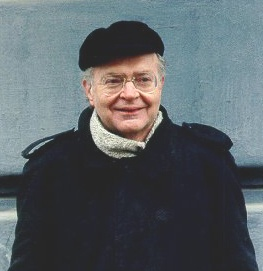
\includegraphics[width=0.6\linewidth]{images/knuth}
    \caption{Knuth}
    \label{fig:my_label2}
\end{figure}



\paragraph*{Актуальность.}

\paragraph*{Цель исследования.}
\paragraph*{Научные задачи.}

\paragraph*{Методы исследования.}


\paragraph*{Основные положения, выносимые на защиту.}
\paragraph*{Научная новизна.}
\paragraph*{Практическая значимость.}
\paragraph*{Достоверность.}
\paragraph*{Аппробация работы.}
\paragraph*{Личный вклад автора.}
\paragraph*{Публикации.}
\paragraph*{Объём и структура работы.}
Диссертация состоит из~введения,
\formbytotal{totalchapter}{глав}{ы}{}{},
заключения и
\formbytotal{totalappendix}{приложен}{ия}{ий}{}.
%% на случай ошибок оставляю исходный кусок на месте, закомментированным
%Полный объём диссертации составляет  \ref*{TotPages}~страницу
%с~\totalfigures{}~рисунками и~\totaltables{}~таблицами. Список литературы
%содержит \total{citenum}~наименований.
%
Полный объём диссертации составляет
\formbytotal{TotPages}{страниц}{у}{ы}{}, включая
\formbytotal{totalcount@figure}{рисун}{ок}{ка}{ков} и
\formbytotal{totalcount@table}{таблиц}{у}{ы}{}.
Список литературы содержит
\formbytotal{citenum}{наименован}{ие}{ия}{ий}.


\newpage
\section*{Основное содержание работы}




%\section*{Список публикаций}
%%
%% Список публикаций
%%
\ifdefmacro{\microtypesetup}{\microtypesetup{protrusion=false}}{} % не рекомендуется применять пакет микротипографики к автоматически генерируемому списку литературы
\urlstyle{rm}                               % ссылки URL обычным шрифтом
% Реализация пакетом biblatex через движок biber
% Цитирования.
%  * Порядок перечисления определяет порядок в библиографии (только внутри подраздела, если `\insertbiblioauthorgrouped`).
%  * Если не соблюдать порядок "как для \printbibliography", нумерация в `\insertbiblioauthor` будет кривой.
%  * Если цитировать каждый источник отдельной командой --- найти некоторые ошибки будет проще.
%
%% authorvak
\nocite{vakbib1}%
\nocite{vakbib2}%
%
%% authorwos
\nocite{wosbib1}%
%
%% authorscopus
\nocite{scbib1}%
%
%% authorpathent
\nocite{patbib1}%
%
%% authorprogram
\nocite{progbib1}%
%
%% authorconf
\nocite{confbib1}%
\nocite{confbib2}%
%
%% authorother
\nocite{bib1}%
\nocite{bib2}%

\insertbiblioauthorgrouped

% \ifnum \totvalue{citeexternal}>0
%     \begin{refcontext}[labelprefix=A]
%         \ifnum \value{bibgrouped}>0
%             \insertbiblioauthorgrouped    % Вывод всех работ автора, сгруппированных по источникам
%         \else
%             \insertbiblioauthor      % Вывод всех работ автора
%         \fi
%     \end{refcontext}
% \else
%     \ifnum \value{bibgrouped}>0
%         \insertbiblioauthorgrouped    % Вывод всех работ автора, сгруппированных по источникам
%     \else
%         \insertbiblioauthor      % Вывод всех работ автора
%     \fi
% \fi

%  \insertbiblioauthorimportant  % Вывод наиболее значимых работ автора (определяется в файле characteristic во второй section)
\begin{refcontext}[labelprefix={}]
    \insertbiblioexternal            % Вывод списка литературы, на которую ссылались в тексте автореферата
\end{refcontext}
% Невидимый библиографический список для подсчёта количества внешних публикаций
% Используется, чтобы убрать приставку "А" у работ автора, если в автореферате нет
% цитирований внешних источников.
\printbibliography[heading=nobibheading, section=0, env=countexternal, keyword=biblioexternal, resetnumbers=true]%


\ifdefmacro{\microtypesetup}{\microtypesetup{protrusion=true}}{}
\urlstyle{tt}                               % возвращаем установки шрифта ссылок URL % реферат на русском
\chapter*{Synopsis}
\addcontentsline{toc}{chapter}{Synopsis} 

\begin{center}
    General thesis summary
\end{center}


\paragraph*{Relevance of the chosen topic.}
\paragraph*{Goal.}
\paragraph*{Objectives.}
\paragraph*{Research methods.}
\paragraph*{Assertions that are presented for defense.}
\paragraph*{The novelty of research.}
\paragraph*{The scientific and technical objective.}
\paragraph*{The research object.}
\paragraph*{The research subject.}
\paragraph*{The theoretical significance.}
\paragraph*{The practical significance.}
\paragraph*{The accuracy of the obtained results.}

\paragraph*{Implementation of research results.}
\paragraph*{Approbation of research results.}
\paragraph*{Personal contribution of the author.}
\paragraph*{Thesis structure and number of pages.}

\newpage
\section*{Main contents of the work}

In Chapter~\ref{ch:ch1}...

\section*{Publications.}

Key results of research are described in \theAllMyPapers~publications. 
Among them
%Four of them are published in journals recommended by the Higher Attestation Commission,
\theScopusPapers~is published in a journal indexed by Scopus. 
%One certificate of state registration of a computer program has also been obtained.



Publications in international journals indexed by Scopus:
\begin{refsection}[biblio/own.bib]
\nocite{*}
\printbibliography[
    keyword=scopus,
    %title={В международных изданиях, индексируемых в базе данных Scopus}, 
    %heading=subbibliography,
    heading=none,
    resetnumbers=true
]
\end{refsection}


List of all relevant author's publications:
\begin{refsection}[biblio/own.bib]
\nocite{*}
\printbibliography[
    keyword=own,
    %title={Список всех публикаций автора по теме диссертации}, 
    %heading=subbibliography,
    heading=none,
    resetnumbers=true
]
\end{refsection} % реферат на английском
\chapter*{Введение}                         % Заголовок
\addcontentsline{toc}{chapter}{Введение}    % Добавляем его в оглавление

В современном мире данные все чаще представляются и хранятся в виде графов, которые часто используются в специализированных базах данных. Для извлечения информации из таких графов обычно применяются строковые языки запросов, однако данный подход имеет свои недостатки. В данной работе представлен подход к поиску путей в графе с ограничениями, основанный на использовании парсер-комбинаторов.

Целью данной работы является разработка библиотеки на языке Kotlin, которая позволит задавать ограничения на поиск путей в графе путем описания грамматики через комбинаторы. Реализация библиотеки включает в себя различные алгоритмы, обеспечивающие оптимальную скорость работы, поддержку недетерминированных и леворекурсивных грамматик, а также обнаружение циклов в графе. Предложенный подход решает ряд проблем, существующих у аналогов с парсер-комбинаторами.

В данной работе проведен сравнительный анализ времени работы разработанного решения и существующей библиотеки Meerkat, которая является наиболее быстрой библиотекой парсер-комбинаторов на данный момент.     % Введение

\ifnumequal{\value{contnumfig}}{1}{\counterwithout{figure}{chapter}
}{\counterwithin{figure}{chapter}}
\ifnumequal{\value{contnumtab}}{1}{\counterwithout{table}{chapter}
}{\counterwithin{table}{chapter}}

\chapter{Оформление различных элементов}
\label{ch:ch1}

\begin{figure}
    \centering
    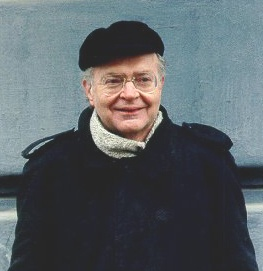
\includegraphics[width=0.6\linewidth]{images/knuth}
    \caption{Knuth}
    \label{fig:my_label4}
\end{figure}


\section{Форматирование чисел и размерностей величин}\label{sec:units}

Числа форматируются при помощи команды \verb|\num|:
\num{5,3};
\num{2,3e8};
\num{12345,67890};
\num{2,6 d4};
\num{1+-2i};
\num{.3e45};
\num[exponent-base=2]{5 e64};
\num[exponent-base=2,exponent-to-prefix]{5 e64};
\num{1.654 x 2.34 x 3.430}
\num{1 2 x 3 / 4}.


Обратите внимание, что ГОСТ запрещает использование знака <<->> для обозначения отрицательных чисел
за исключением формул, таблиц и~рисунков.
Вместо него следует использовать слово <<минус>>.

Размерности можно записывать при помощи команд \verb|\si| и \verb|\SI|:
\si{\farad\squared\lumen\candela};
\si{\joule\per\mole\per\kelvin};
\si[per-mode = symbol-or-fraction]{\joule\per\mole\per\kelvin};
\si{\metre\per\second\squared};
\SI{0.10(5)}{\neper};
\SI{1.2-3i e5}{\joule\per\mole\per\kelvin};
\SIlist{1;2;3;4}{\tesla};
\SIrange{50}{100}{\volt}.

\begin{table}
    \centering
    \captionsetup{justification=centering} % выравнивание подписи по-центру
    \caption{Основные величины СИ}\label{tab:unit:base}
    \begin{tabular}{llc}
        \toprule
        Название  & Команда                 & Символ         \\
        \midrule
        Ампер     & \verb|\ampere| & \si{\ampere}   \\
        Кандела   & \verb|\candela| & \si{\candela}  \\
        Кельвин   & \verb|\kelvin| & \si{\kelvin}   \\
        Килограмм & \verb|\kilogram| & \si{\kilogram} \\
        Метр      & \verb|\metre| & \si{\metre}    \\
        Моль      & \verb|\mole| & \si{\mole}     \\
        Секунда   & \verb|\second| & \si{\second}   \\
        \bottomrule
    \end{tabular}
\end{table}

           % Глава 1
\chapter{Цель и задачи}
\label{ch:ch2}

\section{Цель}
В итоге была сформулирована следующая цель работы: разработать библиотеку комбинаторов запросов к графам
на основе алгоритмов, предложенных в работе \cite{Meerkat}. При этом нужно разработать такую архитектуру комбинаторов и парсера, чтобы исправить проблемы Meerkat.
\section{Задачи}
\begin{enumerate}
    \item Разработать базовую структуру парсера и комбинаторов;
    \item Поддержать левую рекурсию путем мемоизации результатов парсера;
    \item Поддержать циклы, генерируя SPPF;
    \item Реализовать извлечение результатов из SPPF;
    \item Сравнить скорость работы с другими решениями.
\end{enumerate} 
           % Глава 2
\chapter{Реализация библиотеки парсер-комбинаторов}
\label{ch:ch3}

В качестве языка программирования для реализации библиотеки парсер-комбинаторов был взят Kotlin.
Он поддерживает функции высшего порядка, а также имеет удобный синтаксис для анонимных функций.
Помимо этого он поддерживает функции в инфиксной нотации, что будет удобно для комбинирования парсеров.


\section{Базовая структура парсера}

Изначально была разработана базовая архитектура библиотеки, комбинаторы в которой были реализованы через рекурсивный спуск.
Такие комбинаторы вызывали другие рекурсивно, что могло привести к бесконечному выполнению на графах с циклами или при наличии левой рекурсии в определении парсера.
Даже без таких особенностей мы могли получить переполнение стека вызовов на достаточно объемном входе.
Но данный подход обладает простотой реализации, что позволяет относительно быстро разработать базовую архитектуру и различные комбинаторы.

Рассмотрим тип парсера, который был изначально разработан, но в последствии изменен при реализации алгоритмов:
\begin{lstlisting}
BaseParser<I, O, R>(
    val f: (I) -> Sequence<ParserResult<O, R>>)
\end{lstlisting}
За основу был взят тип из библиотеки Trails. Парсер параметризуется тремя типами: типы входящего и выходящего состояния и тип результата.

Парсер по сути является функцией, которая принимает входящее состояние и возвращает последовательность выходящих состояний и результатов. В данном случае \verb|ParserResult| представляет из себя пару. Класс \verb|Sequence| - это стандартная структура данных в Kotlin, которая представляет из себя ленивую последовательность, которая вычисляется в процессе извлечения из нее данных. Здесь \verb|Sequence| используется из-за того, что результатов может быть бесконечно много, например, при наличии циклов в графе, а \verb|Sequence| позволяет лениво извлекать эти результаты.

В Trails вместе с входящим состоянием передается окружение, которое как-то связанно с этим состоянием, например, это можем быть граф или строка. В моем решении это окружение содержится внутри самого состояния.

В контексте работы с графами я ввел три различных типа состояний: стартовое состояние, состояние на ребре и состояние на вершине. Стартовое состояние обозначает, что парсер принимает весь граф, и может начать разбор с любой вершины или ребра. Состояние на ребре хранит конкретное ребро, с которого нужно продолжить разбор. Аналогично про состояние на вершине. Все эти состояния хранят ссылку на граф, с которым они ассоциированы.

Чтобы работать с различными реализациями графов, я написал интерфейс графа, которому эти реализации должны соответствовать. Этот интерфейс будут использовать базовые комбинаторы графа, описанные в следующем разделе.

\section{Парсер-комбинаторы}

\subsection{Базовые комбинаторы для графа}

Рассмотрим базовые комбинаторы для разбора графа, из которых с помощью других комбинаторов будут конструироваться сложные запросы.

Чтобы создать парсер, который будет принимать стартовое состояние, используются комбинаторы \verb|v| и \verb|edge|:

\begin{nobreaks}
    \begin{lstlisting}
fun v(p: (V) -> Boolean = { true })
    : BaseParser<StartState<V, E>, VertexState<V, E>, V>
fun edge(p: (E) -> Boolean = { true })
    : BaseParser<StartState<V, E>, EdgeState<V, E>, E> 
\end{lstlisting}
\end{nobreaks}

Функция \verb|v| принимает предикат, по которому все множество вершин графа фильтруется, и каждая подходящая вершина возвращается как выходящее состояние и результат.
Аналогично функция \verb|edge|.
Для этих парсеров интерфейс графа содержит методы для получения последовательности всех вершин и ребер.

Для случая, когда мы получаем состояние на вершине и хотим разобрать входящие или исходящие ребра, мы можем воспользоваться следующими комбинаторами:

\begin{nobreaks}
\begin{lstlisting}
fun outE(p: (E) -> Boolean = { true })
    : BaseParser<VertexState<V, E>, EdgeState<V, E>, E>
fun inE(p: (E) -> Boolean = { true })
    : BaseParser<VertexState<V, E>, EdgeState<V, E>, E>
\end{lstlisting}
\end{nobreaks}

Функции \verb|outE| и \verb|inE| принимают предикат, по которому фильтруют множества исходящих или входящих ребер текущей вершины. Соответственно, возвращают такие парсеры состояния на ребрах и сами ребра как результаты.

Если мы находимся на ребре и хотим разобрать начальную или конечную вершину этого ребра, то можно использовать аналогичные комбинаторы \verb|outV| и \verb|inV|:
\begin{lstlisting}
fun outV(p: (V) -> Boolean = { true })
    : BaseParser<EdgeState<V, E>, VertexState<V, E>, V>
fun inV(p: (V) -> Boolean = { true })
    : BaseParser<EdgeState<V, E>, VertexState<V, E>, V>
\end{lstlisting}

Интерфейс графа, для поддержки комбинаторов вершин и ребер, должен позволять получать множество входящих или исходящий ребер для конкретной вершины, а также получать начальную или конечную вершину для конкретного ребра.

Также были добавлены более общие базовые комбинаторы: \verb|success|, \verb|eps| и \verb|fail|.
Комбинатор \verb|success| создает парсер, который возвращает переданный аргумент как результат разбора, не изменяя входящее состояние.
Комбинатор \verb|eps| -- частный случай \verb|success|, возвращающий \verb|Unit|\footnote{В других языках данный тип называют \texttt{void}}.
Комбинатор \verb|fail| создает парсер, не возвращающий результатов и не изменяющий состояние.
Их сигнатуры следующие:
\begin{lstlisting}
fun success(v: R): BaseParser<S, S, R>  
fun eps(): BaseParser<S, S, Unit>
fun fail(): BaseParser<S, S, R>
\end{lstlisting}

Базовая структура парсера, описанная в предыдущем разделе, позволяет создавать не только парсеры для графов, но и для строк.
В рамках тестирования полученной архитектуры были разработаны комбинаторы для создания строковых парсеров.
Они позволяют создавать парсеры из строки или регулярного выражения.

\begin{lstlisting}[float=ht, label=lst:stringParser, caption=Пример строкового парсера]
val expr = LazyParser<StringPos, StringPos, Int>()
expr.p = rule(
    (expr seql "+".p seq expr) using { x, y -> x + y },
    (expr seql "−".p seq expr) using { x, y -> x - y },
    "(".p seqr expr seql ")".p,
    "[0−9]*".toRegex().p using { it.toInt() })
\end{lstlisting}

В листинге \ref{lst:stringParser} мы создаем парсер, способный разбирать и вычислять арифметические выражения с операциями \verb|+|, \verb|-| и группирующими скобками.


\subsection{Объединяющие комбинаторы}

Рассмотрим реализованные в рамках этой работы комбинаторы для объединения парсеров.

\begin{lstlisting}[float=ht, label=lst:combinators, caption=Объединяющие комбинаторы]
fun BaseParser<I, O1, R1>.seq(p2: BaseParser<O1, O2, R2>)
                : BaseParser<I, O2, Pair<R1, R2>>

fun BaseParser<I, O, R>.or(p2: BaseParser<I, O, R>)
                : BaseParser<I, O, R>

fun BaseParser<I, O, A>.using(f: (A) -> B): BaseParser<I, O, B>

fun BaseParser<I, O, R>.that(constraint: BaseParser<O, O2, R2>)
                : BaseParser<I, O, R> 

val BaseParser<S, S, R>.many: BaseParser<S, S, List<R>>
val BaseParser<S, S, R>.some: BaseParser<S, S, List<R>>
\end{lstlisting}

Комбинатор \verb|seq| (листинг \ref{lst:combinators}) позволяет объединить два парсера последовательно, так, что выходящие состояния первого парсера передаются во второй.
Результаты же обоих парсеров объединяются в пару.
Также реализованы специальные комбинаторы \verb|seql| и \verb|seqr|, которые действуют как \verb|seq|, но возвращают только левый или правый результат. Это может быть полезно, когда мы хотим проигнорировать какие-то ключевые слова в тексте или определенные вершины в графе. Пример использования таких комбинаторов можно увидеть в листинге \ref{lst:stringParser}: они использовались для игнорирования строкового представления операторов и скобок.

Комбинатор \verb|or| (листинг \ref{lst:combinators}) позволяет объединить два парсера параллельно.
Результирующий парсер будет передавать входящее состояние в оба парсера и объединять их результаты и выходящие состояния.
Поэтому оба парсера должны принимать и возвращать одинаковые типы состояний и результата.

Комбинатор \verb|or| обычно используется чтобы описать несколько парсеров у одного правила в грамматике, но для этого нужно оборачивать каждый парсер в скобки, т.к. в Kotlin нельзя задать приоритет объявленной инфиксной операции. Именно для этого был введен метод \verb|rule|, который принимает любое количество парсеров как аргументы, и возвращает их параллельное объединение. Пример использования \verb|rule| приведен в листинге \ref{lst:stringParser}.

Следующий комбинатор -- это \verb|using| (листинг \ref{lst:combinators}), которая является альтернативой функции \texttt{map} из библиотеки Trails. Эта функция позволяет заменить результаты парсера на другие с помощью функции \verb|f|.
Для этого он создает новый парсер, который внутри реализует эту логику, сохраняя исходный парсер и функцию \verb|f|.

Но иногда \verb|using| применяется к последовательности парсеров.
Например, возьмем такой парсер:

\begin{nobreaks}
    \begin{lstlisting}
(v() seq outE() seq outV()) using { (tmp, u) -> 
    val (v, e) = tmp
    ... 
}
\end{lstlisting}
\end{nobreaks}

Мы знаем, что \verb|seq| создает парсер, который возвращает пару результатов, соответственно парсер выше возвращает \verb|Pair<Pair<V, E>, V>|.
В Kotlin, к сожалению, нет вложенного деструктурирования, чтобы достать обе вершины и ребро за один раз.
Если мы хотим деструктурировать такой результат, нам бы пришлось делать это дважды, как в примере выше, что неудобно.
Для решения это проблемы добавлены перегрузки функции \verb|using|, отличающиеся типом результата у парсера, а именно, когда парсер возвращает вложенные пары. Такие перегрузки принимают функцию \verb|f| с арностью больше один. С ними пример выше можно переписать так:
\begin{lstlisting}
(v() seq outE() seq outV()) using { v, e, u -> ... }
\end{lstlisting}

Другим подходом для решения этой проблемы могли бы быть перегрузки комбинатора \verb|seq|, которые бы объединяли пары результатов в кортежи, которые уже можно деструктурировать за один раз. Проблема тут в том, что в Kotlin нет поддержки кортежей, из-за чего нужно было бы самостоятельно определить типы кортежей разной длины.

В строковых языках запросов часто используется блок \texttt{where} для задания определенных ограничений. Чтобы частично реализовать такое поведение, был введен комбинатор \texttt{that} (листинг \ref{lst:combinators}). Его сигнатура похожа на комбинатор \texttt{seq}: он также принимает два парсера, где второй применяется к результатам первого. Но возвращается парсер, который действует также, как и первый, но результаты которого отфильтрованы. В роли предиката выступает второй парсер: результат отбрасывается, если второй парсер на нем не вернул ни одного результата. Второй парсер также можно назвать подзапросом.


\begin{lstlisting}[float=ht, label=lst:marysLover, caption={Пример запроса к графу с комбинатором \texttt{that}}]
val person = v()
val isMary = vPred { v -> v.value == "Mary" }
val isLoves = ePred { e -> e.label == "loves" }
val marysLover = person
            .that(outE(isLoves) seq outV(isMary))
            .that(inE(isLoves) seq inV(isMary))
val friend = outE { it.label == "friend" }
val marysLoversFriend = marysLover seqr friend seqr outV()
\end{lstlisting}

Пример использования комбинатора \texttt{that} приведен в листинге \ref{lst:marysLover}. В нем мы находим всех людей, которые любят Мэри и Мэри любит их в ответ. После чего для всех таких людей мы находим их друзей. Написать такую логику без комбинатора \texttt{that} было бы сложно, так как другие комбинаторы меняют состояние исходного парсера, а комбинатор \texttt{that} -- нет.

Чтобы писать парсеры циклов, мы можем использовать комбинатор \texttt{many} (листинг \ref{lst:combinators}).
В качестве аргумента он принимает парсер, который имеет одинаковый тип входящего и выходящего состояния.
Этот комбинатор создает парсер, который действует как переданный, но последовательно объединенный сам с собой ноль и более раз.
Созданный парсер возвращает списки результатов длины \texttt{k}, где \texttt{k} -- количество последовательных повторений исходного парсера.
Также написан аналогичный комбинатор \texttt{some}, но для повторений от одного и более раз.

Следующей проблемой является описание рекурсивных парсеров. В Kotlin нельзя использовать переменную в ее же инициализации. А для взаимно-рекурсивных определений мы не можем использовать переменную, которая будет объявлена дальше по коду.

Подход, который предлагается в работе \cite{Meerkat}, заключается в использовании комбинатора неподвижной точки.
Он позволяет инициализировать парсер, используя в определении этот же парсер. Вот пример использования:
\begin{lstlisting}
val s = fix { s -> ("a".p seql s).many }
\end{lstlisting}
Комбинатор \texttt{fix} принимает функцию, которая возвращает парсер, инициализированный с использованием  аргумента \texttt{s}. Этот аргумент является тем самым парсером, который эта функция создает.
Тип комбинатора \texttt{fix} выглядит так:

\begin{nobreaks}
    \begin{lstlisting}
fun fix(f: (BaseParser<I, O, R>) -> BaseParser<I, O, R>)
    : BaseParser<I, O, R>
\end{lstlisting}
\end{nobreaks}

Использование комбинатора \texttt{fix} имеет свои недостатки: нужно дублировать имя переменной и нельзя объявить взаимно-рекурсивные парсеры. Для взаимной рекурсии можно создать другие определения \texttt{fix}, которые будут принимать функции с арностью больше один. Тогда такая функция должна возвращать столько же парсеров, сколько и аргументов она получает, при этом каждое определение парсера соответствует своему аргументу. А учитывая, что в Kotlin нет удобной поддержки кортежей, такой подход будет неудобным.

Для решения проблемы с взаимно-рекурсивным определением, я добавил парсеры с отложенной инициализацией, названные \texttt{LazyParser}. Использование такого парсера можно увидеть в листинге \ref{lst:stringParser}. Такой подход больше соответствует императивному стилю программирования, что может быть удобным для некоторых пользователей. Также с помощью таких парсеров мы можем определить взаимно-рекурсивные парсеры, например, сначала объявив нужные парсеры, а затем инициализировав их. Но у данного подхода есть проблема: проверка того, что парсер был инициализирован, происходит только во время исполнения, а не во время компиляции. У комбинатора \texttt{fix} такой проблемы нет: мы не можем создать парсер, не инициализировав его. К сожалению, в случае \texttt{LazyParser}, мы не можем с помощью системы типов определить, был ли парсер инициализирован.





\section{Мемоизация состояний и результатов}

Как упоминалось ранее, комбинаторы, реализованные через рекурсивный спуск, не способны поддерживать левую рекурсию в определении грамматики, а также циклы в графе.

\begin{lstlisting}[float=ht, label=lst:leftRec, caption=Пример левой рекурсии в грамматике]
    val s = fix { s -> s seq outE() seq outV() or eps() }
\end{lstlisting}

В качестве примера возьмем код с листинга \ref{lst:leftRec}. Допустим, в комбинаторе \texttt{or} мы сначала вызываем первый парсер. Комбинатор \texttt{seq} определен так, что он сначала вызывает первый парсер и на каждом его результате вызывает второй. Таким образом, при вызове парсера \texttt{s}, мы рекурсивно спускаемся до этого же парсера \texttt{s}, и этот процесс будет повторятся бесконечно.

Для решения проблемы, описанной выше, мы хотим детектировать случаи, когда мы рекурсивно спустились в тот же парсер. Для этого добавим мемоизацию на уровне парсера.

Давайте для каждого входящего состояния запоминать результат, который мы возвращали для него ранее. Тогда при повторении входящего состояния для парсера, мы не будем снова вычислять результат, а вернем тот, который запомнили ранее.

Но какой результат возвращать при первом вызове парсера \texttt{s} в листинге \ref{lst:leftRec}?
Его сначала нужно вычислить, но это приведет к рекурсивному вызову.
Тут можно воспользоваться идеей из работы \cite{MemoizationJohnson} в использовании стиля передачи продолжений (Continuation-Passing Style, CPS) при определении парсера.

Обычная функция в привычном понимании при вызове с некоторыми аргументами возвращает результат. Функция \texttt{f}, написанная в CPS стиле, вместе c аргументами принимает продолжение (continuation) и не возвращает результат. Продолжение само по себе является функцией, которая принимает результат функции \texttt{f}. Функция \texttt{f} при вычислении передает свои результаты в продолжение. Продолжение представляет из себя некоторое вычисление, которое как-то обрабатывает каждый результат функции \text{f}.

\begin{lstlisting}[float=ht, label={lst:CpsExample}, caption=Пример функции в CPS стиле]
fun foo(x: A, y: B): List<R> {
    return listOf(x.bar(y), x.baz())
}

fun fooCPS(x: A, y: B, c: (R) -> Unit): Unit {
    c(x.bar(y))
    c(x.baz())
}
\end{lstlisting}

Например, в листинге \ref{lst:CpsExample} функция \texttt{foo} написана в обычном стиле, и она возвращает несколько результатов как список. Такую функцию можно переписать, используя CPS стиль, получив в итоге функцию \texttt{fooCPS}, которая каждый результат передает в продолжение \texttt{c}.

Как было сказано ранее, парсер является функцией, которая принимает входящее состояние, производит некоторое вычисление и возвращает множество пар выходящих состояний и результатов. Мы хотим для каждого входящего состояния запоминать результат работы парсера. Пусть тогда парсер вместо непосредственно результатов возвращает некоторое вычисление и запоминает его.

Это вычисление будет является функцией, написанной в стиле передачи продолжений. Назовем это вычисление \texttt{ParserResult}. Тогда оно будет определено так:

\begin{lstlisting}[float=ht]
typealias Continuation<S, R> = (S, R) -> Unit
class ParserResult<S, R>(
        val f: (Continuation<S, R>) -> Unit) {...}
\end{lstlisting}

Это вычисление будет представлять из себя работу парсера. При этом каждые вычисленные результат и выходящее состояние будут передаваться в продолжение.

Теперь парсер может для каждого входящего состояния запоминать вычисление, которое он вернул, чтобы возвращать ту же функцию в следующий раз. Теперь нам нужно обеспечить, чтобы это вычисление исполнялось один раз.

\begin{lstlisting}[language=Matlab, label={lst:memoResult}, float=ht, caption=Мемоизация результата парсера]
function memoResult(parserRes):
results = empty list of pairs (S, R)
continuations = empty list of Continuation<S, R>

return function (k):
    isFirstCall = continuations is empty
    add k to continuations
    
    if isFirstCall:
        parserRes.apply(function (s, r):
            newResult = (s, r)
            if newResult not in results:
                add newResult to results
                for each continuation in continuations:
                    continuation(s, r))   
    else:
        for each (s, r) in results:
            k(s, r)
\end{lstlisting}

Для этого обернем вычисление, которое возвращает парсер, в другое вычисление, которое будет обеспечивать единственность выполнения.
Псевдокод функции \texttt{memoResult}, которая это делает, представлен в листинге \ref{lst:memoResult}.

Будем для вычисления парсера хранить список результатов, которые он вернул, и список продолжений, с которыми это вычисление вызывали. Когда вычисление парсера впервые вызывают, список с продолжениями пуст. Тогда мы и будем впервые исполнять исходное вычисление. Как известно, оно принимает продолжение, поэтому мы создадим свое продолжение и передадим его. В нем мы будем получать выходящие состояния и результаты парсера на текущем входящем состоянии. Если такой результат мы не получали ранее, то передадим его всем продолжениям, которые мы запомнили.

Если вычисление вызывается повторно, то мы не будем исполнять исходное вычисление парсера, а просто передадим в полученное продолжение все известные на данный момент результаты, при этом сохранив это продолжение на случай, если в будущем появятся новые результаты.

Рассмотрим выполнение парсера \texttt{s} в листинге \ref{lst:leftRec} с такой реализацией парсера.
Когда мы впервые вызываем парсер \texttt{s}, мы передаем в него продолжение, которое будет принимать его результаты.
Это продолжение мы запоминаем, и вызываем вычисление парсера \texttt{s}.
Там мы рекурсивно спустимся в левую ветку \texttt{or}, пройдем через пару \texttt{seq} и снова вызовем парсер \texttt{s}.
На этот раз мы будем вызывать его с продолжением, в котором будет вызываться следующий за ним парсер \texttt{outE()} в последовательности \texttt{s seq outE() seq outV()}.
На этот момент парсер \texttt{s} не запомнил ни одного результата, поэтому переданное продолжение вызвано не будет, но оно будет запомнено.
Далее мы вернемся на уровень комбинатора \texttt{or}, и вызовем правый парсер.
Там находится комбинатор \texttt{eps}, который всегда возвращает результат \texttt{Unit}.
Этот \texttt{Unit} будет возвращен как результат парсера \texttt{s}.
Получим этот результат мы в вычислении, которое сохранили в функции \texttt{memoResult}, где на данный момент запомнили два продолжения.
Когда этот результат будет передаваться в первое продолжение, его получит пользователь парсера \texttt{s}.
Когда же он будет передаваться во второе продолжение, его получит парсер \texttt{outE()}, следующий за парсером \texttt{s}.
Если в графе есть путь с исходящим ребром и вершиной, то парсер \texttt{s} вернет еще один результат, который также будет передан в два сохраненных продолжения.
Это будет продолжаться до тех пор, пока в графе есть подходящие грамматике пути.

Так мы смогли поддержать леворекурсивные грамматики.
А также такая реализация парсера, описанная в работе \cite{MemoizationJohnson}, улучшает скорость работы разбора с экспоненциальной до полиномиальной.
Но что, если в графе будет цикл?
Тогда путей, соответствующих грамматике, будет бесконечно много, и вычисление парсера \texttt{s} будет бесконечным.

\section{Сжатый лес разбора}

Для решения проблемы с бесконечным количеством результатов парсер должен возвращать некоторую конечную структуру данных, которая может представлять все возможные разборы парсера.

\begin{figure}[t]
    \centering
    \begin{subfigure}[b]{0.25\textwidth}
        \centering
        \includesvg[inkscapelatex=false,width=\textwidth]{sppf/gr.svg}
        \caption{Граф}
        \label{fig:subGraph}
    \end{subfigure}
    \hfill
    \begin{subfigure}[b]{0.55\textwidth}
        \centering
        \includesvg[inkscapelatex=false,width=\textwidth]{sppf/1.svg}
        \caption{Первое дерево разбора}
        \label{fig:subDerivedTrees1}
    \end{subfigure}
    \vskip\baselineskip
    \begin{subfigure}[b]{1.00\textwidth}
        \centering
        \includesvg[inkscapelatex=false,width=\textwidth]{sppf/2.svg}
        \caption{Второе дерево разбора}
        \label{fig:subDerivedTrees2}
    \end{subfigure}


    \caption{Пример деревьев разбора}
    \label{fig:derivedTrees}
\end{figure}

\begin{figure}[t]
    \centering
    \begin{subfigure}[b]{0.8\textwidth}
        \centering
        \includesvg[inkscapelatex=false,width=\textwidth]{sppf/3.svg}
        \caption{SPPF}
        \label{fig:subSppf}
    \end{subfigure}
    \hfill
    \begin{subfigure}[b]{0.7\textwidth}
        \centering
        \includesvg[inkscapelatex=false,width=\textwidth]{sppf/4.svg}
        \caption{Бинаризованный SPPF}
        \label{fig:subBinSppf}
    \end{subfigure}

    \caption{Пример обычного и бинаризованного SPPF}
    \label{fig:sppf}
\end{figure}


Такой структурой может являться сжатое представление леса разбора (Shared Packed Parse Forest, SPPF). Впервые такая структура была использована в работе \cite{RekersSppf}.

Рассмотрим пример разбора графа, изображенного на рисунке \ref{fig:subGraph}. Разбор проводился с помощью парсера \texttt{S} в листинге \ref{fig:sppfParser}.

\begin{lstlisting}[float=h, label=fig:sppfParser, caption=Пример парсера для разбора графа]
val x = outV { it.value == "x" }
val y = outV { it.value == "y" }
val a = outE { it.label == "A" }
val b = outE { it.label == "B" }
val P = a seq y
val S = P or (P seq b seq y)
\end{lstlisting}

Парсер запускался, начиная с вершины \texttt{x}. На рисунке \ref{fig:subDerivedTrees1} и \ref{fig:subDerivedTrees2} изображены два дерева разбора. В них листья соответствуют базовым комбинаторам, а остальные - объединяющим комбинаторам. Вершина в дереве имеет вид $(p, i, o)$, где $p$ - парсер или результат, $i$ - входящее состояние, $o$ - выходящее состояние. Первое дерево соответствует пути $x \xrightarrow{A} y$, а второе -- пути $x \xrightarrow{A} y \xrightarrow{B} y$.

Таких деревьев разбора может быть бесконечно много, но мы можем объединить их в SPPF. Пример SPPF для упомянутых ранее деревьев разбора приведен на рисунке \ref{fig:subSppf}. В этом представлении появляется новый тип сжатых вершин, на рисунке изображенный небольшим квадратом. Такая вершина представляет из себя один из вариантов разбора родительской вершины. На рисунке \ref{fig:subSppf} видим, что некоторые вершины присутствуют в обоих разборах, например, вершина \texttt{E("A")}.

В работе \cite{BinSppf} было представлено бинаризованное SPPF, что является улучшением обычного SPPF. В бинаризованном виде объем леса достигается $O(n^3)$, где $n$ - размер графа. В таком SPPF сжатые узлы имеют не более двух детей. Пример сжатого леса разбора приведен на рисунке \ref{fig:subBinSppf}.

Как мы можем заметить, узел SPPF параметризуется парсером, входящим и выходящим состоянием. Даже если у нас будет бесконечное количество деревьев разбора, у нас будет конечный объем SPPF, т.к. количество парсеров и состояний конечно.

\begin{figure}[htp]
    \centering
    \begin{subfigure}[b]{0.3\textwidth}
        \centering
        \includesvg[inkscapelatex=false,width=0.5\textwidth]{sppf/loop_gr.svg}
        \caption{Граф}
        \label{fig:subLoopGr}
    \end{subfigure}
    \hfill
    \begin{subfigure}[b]{0.5\textwidth}
        \centering
        \includesvg[inkscapelatex=false,width=\textwidth]{sppf/loop.svg}
        \caption{SPPF}
        \label{fig:subLoopSppf}
    \end{subfigure}

    \caption{Пример SPPF с циклом}
    \label{fig:sppf}
\end{figure}

Примером случая, когда разбор возвращает бесконечно много результатов, может быть разбора цикла в графе. Возьмем грамматику в листинге \ref{lst:loopParser}.

\begin{lstlisting}[float=h, label={lst:loopParser}, caption=Пример парсера графа с циклом]
val x by outV { it.value == "x" }
val a by outE { it.label == "A" }
val S by LazyParser<SimpleVertexState, SimpleVertexState, Any>()
S.p = (S seq a seq x) or eps()
\end{lstlisting}

Такая грамматика разбирает бесконечно много путей вида $(x \xrightarrow{A} x)*$ в графе на рисунке \ref{fig:subLoopGr}. Лес разбора для такого парсера и графа изображен на рисунке \ref{fig:subLoopSppf}. Как мы можем увидеть, дочерний узел \texttt{(S a)} ссылается на предка \texttt{S}, формируя цикл в SPPF. Такой лес разбора хранит бесконечное количество путей.

\subsection{Генерация сжатого леса разбора}

Чтобы генерировать SPPF как результат разбора, мы должны в вычислении парсера вместо пары <<результат и выходящее состояние>> возвращать вершину SPPF. Рассмотрим, какие вершины будут возвращать комбинаторы.

Все вершины, которые не являются сжатыми, параметризуются начальным и конечным состоянием. Тип несжатой вершины также параметризуется типом результата, который соответствующий ей парсер генерирует:
\begin{lstlisting}
NonPackedNode<LS, RS, R>(val leftState: LS, val rightState: RS)
\end{lstlisting}

Сжатые же вершины хранят ссылку на одного или двух детей, которые в свою очередь являются несжатыми вершинами:

\begin{nobreaks}
    \begin{lstlisting}
class PackedNode<LS, MS, RS, R1, R2>(
    val leftNode: NonPackedNode<LS, MS, R1>?,
    val rightNode: NonPackedNode<MS, RS, R2>
    ...
)
\end{lstlisting}
\end{nobreaks}

Базовые комбинаторы, такие как комбинатор вершины или ребра, генерируют терминальную вершину, которая хранит непосредственно результат: 

\begin{nobreaks}
    \begin{lstlisting}
class TerminalNode<...>(val result: T, val action: (T) -> R, ..)  
    : NonPackedNode<...>(leftState, rightState)
\end{lstlisting}
\end{nobreaks}

Объединяющие комбинаторы генерируют промежуточную вершину. Такая вершина хранит соответствующий парсер, а также список детей, которые являются сжатыми вершинами:

\begin{nobreaks}
\begin{lstlisting}
class IntermediateNode<...>(
    val parser: BaseParser<LS, RS, *>, 
    val action: (Pair<CR1?, CR2>) -> R, ...
) : NonPackedNode<...>(leftState, rightState) {
    val packedNodes: MutableList<PackedNode<..., CR1?, CR2>>
...}
\end{lstlisting}
\end{nobreaks}

Например, комбинатор \texttt{seq} получает две вершины от парсеров и создает промежуточную вершину, к которой через сжатую вершину подвешивает эти две вершины. 

Терминальная и промежуточная вершина также хранят семантическое действие, которое заменяет исходный результат на другой. Такое действие добавляется при использовании комбинатора \texttt{using}. Оно будет использоваться при извлечении результатов из SPPF.

Помимо непосредственной генерации вершин SPPF нам нужно обеспечить раздельное использование одинаковых вершин между парсерами. Упомянутый ранее комбинатор \texttt{seq} должен либо создавать новую промежуточную вершину, либо использовать созданную ранее, чтобы подвесить к ней сжатую вершину. Для этого заведем хранилище вершин, которое будет обеспечивать раздельное доступ к вершинам. Такое хранилище будет представлять из себя множество вершин, которое позволяет добавлять новые вершины в это множество, если таких еще нет, или доставать из него уже созданные ранее вершины. 

Данное хранилище будет передаваться парсеру на вход, а парсер в свою очередь будет передавать его во вложенные парсеры рекурсивно, таким образом все парсеры будут иметь доступ только к одному хранилищу, а значит будут разделять одни и те же вершины. 

\subsection{Извлечение результатов из леса разбора}

Теперь парсер в качестве результата возвращает некоторое количество вершин SPPF, причем конечное. Каждая вершина представляет из себя множество деревьев разбора, причем неограниченного размера.

Для извлечения результатов из SPPF, мы можем совершить его обход, например, в ширину. Такой обход позволяет поддержать возможные циклы в SPPF, но написать извлечение результатов с обходом в ширину не тривиально.

Для простоты реализации был написан обход в глубину, реализованный с помощью структуры данных \texttt{Sequence} из стандартной библиотеки Kotlin, представляющую ленивую последовательность данных. Каждый тип вершины умеет возвращать \texttt{Sequence} результатов. Промежуточная вершина объединяет последовательности результатов сжатых вершин в одну. Терминальная вершина возвращает последовательность из одного элемента, который она хранит. Сжатая вершина возвращает последовательность пар результатов, где каждый результат первого ребенка объединяется с каждым результатом второго ребенка, если второй ребенок есть. 

При этом промежуточная и терминальная вершина перед возвратом каждого результата применяет к нему семантическое действие, которое хранится в вершине. 

Такой обход в глубину был протестирован на графах с циклами, а также на леворекурсивных грамматиках. В итоге не удалось написать такой тест, в котором бы обход в глубину зациклился и не завершился. Это можно объяснить тем, что если в SPPF есть цикл, то обход в глубину на каждой итерации этого цикла будет добавлять ненулевой результат в последовательность. Обход в глубину перебирает сжатые вершины у промежуточной вершины в порядке их добавления. А благодаря мемоизации результатов парсера, первой будет добавляться вершина, которая соответствует той ветви парсера, где нет рекурсивного вызова этого же парсера. Соответственно, из первой сжатой вершины нельзя прийти в цикл. А значит она будет возвращать ненулевой результат, который будет добавлен в последовательность.

           % Глава 3
\chapter{Экспериментальное исследование}
\label{ch:ch4}


Для анализа полученного результата был проведено сравнение времени работы с библиотекой Meerkat. В свою очередь сравнение библиотеки Meerkat c библиотекой Trails приведено в работе \cite{MeerkatGraphs}. Замер производился с помощью фреймворка JMH\footnote{https://github.com/openjdk/jmh (Дата обр. 21.05.2024)}.

Тестирование проводилось на вычислительной машине с 12-ядерным процессором AMD Ryzen 9 7900X и 128 ГБ оперативной памяти DDR5.

Для запуска тестов была добавлена поддержка Neo4j графов, т.к. эту базу данных поддерживает Meerkat. Для этого использовалось предоставляемое Neo4j Java API\footnote{https://neo4j.com/docs/java-reference/4.4/ (дата обр. 21.05.2024)}, с помощью которого был реализован интерфейс графа, с которым работают комбинаторы.

Первый набор тестов был взят такой же, какой использовали авторы расширения Meerkat, в свою очередь он был представлен в работе \cite{RDF_CF}. Это набор онтологий, каждая из которых представлена RDF-файлом. Для тестирования эти файлы были преобразованы в ориентированные графы, каждый из которых был загружен в свою базу данных Neo4j.

\begin{figure}[htp]
    \centering
    \begin{subfigure}[b]{0.49\textwidth}
        \centering
        $Q_1 \to subclassof^{-1}\ Q1?\ subclassof$\\
        $Q_1 \to type^{-1}\ Q1?\ type$\\
        \caption{Запрос 1}
    \end{subfigure}
    \hfill
    \begin{subfigure}[b]{0.49\textwidth}
        \centering
        $S \to subclassof^{-1}\ S?\ subclassof$
        $Q_2 \to S\ subclassof$
        \caption{Запрос 2}
    \end{subfigure}
    \caption{Запросы для тестирования}
    \label{fig:queries}
\end{figure}

Используемые запросы приведены на рисунке \ref{fig:queries}. Ключевые слова, например, \texttt{type} или \texttt{subclassof}, являются метками на ребрах. Верхний индекс \texttt{-1} обозначает обратное направление ребра. Знак \texttt{?} обозначает ноль или одно применение парсера.

\begin{lstlisting}[float=h, label=lst:qqueries, caption={Запросы, используя комбинаторы}]
val subclassof1 = throughInE { it.label == "subClassOf" }
val subclassof = throughOutE { it.label == "subClassOf" }
val type1 = throughInE { it.label == "type" }
val type = throughOutE { it.label == "type" }
val Q1 = LazyParser<Neo4jVertexState, Neo4jVertexState, Any>()
Q1.p = (subclassof1 seq (Q1 or eps()) seq subclassof) or
        (type1 seq (Q1 or eps()) seq type)

val S = LazyParser<Neo4jVertexState, Neo4jVertexState, Any>()
S.p = (subclassof1 seq (S or eps()) seq subclassof)
val Q2 = ((S or eps()) seq subclassof)
\end{lstlisting}

Описание этих запросов, используя комбинаторы, приведено в листинге \ref{lst:qqueries}. Комбинаторы \texttt{throughOutE} и \texttt{throughInE} вспомогательные: они пропускают выходящую или входящую вершину ребра соответственно.

\begin{table}[h]
    \caption{Информация о RDF графах}
    \begin{tabular}{|l|c|c|c|}
        \hline
        \textbf{Граф} & \textbf{Кол-во вершин} & \textbf{Кол-во рёбер} \\
        \hline
        atom-primitive.owl & 291 & 685 \\
        biomedical-measure-primitive.owl & 341 & 711 \\
        foaf.rdf & 256 & 815 \\
        generations.owl & 129 & 351 \\
        people\_pets.rdf & 337 & 834 \\
        pizza.owl & 671 & 2604 \\
        skos.rdf & 144 & 323 \\
        travel.owl & 131 & 397 \\
        univ-bench.owl & 179 & 413 \\
        wine.rdf & 733 & 2450 \\
        \hline
\end{tabular}
\label{tab:rdfGraphs}
\end{table}

Характеристики графов-онтологий приведены в таблице \ref{tab:rdfGraphs}. Результаты замеров приведены в таблице \ref{tab:rdfTimes}. Разработанное решение помечено как GParsers.

\begin{table}[h]
    \caption{Время выполнения на RDF графах}
    \begin{tabular}{|b{0.36\linewidth}|b{0.13\linewidth}|b{0.12\linewidth}|b{0.13\linewidth}|b{0.12\linewidth}|}
        \hline
        \textbf{Граф} & \multicolumn{2}{|c|}{\textbf{Запрос 1 (мс)}} & \multicolumn{2}{|c|}{\textbf{Запрос 2 (мс)}} \\
        \cline{2-5}
         & \textbf{GParsers} & \textbf{Meerkat} & \textbf{GParsers} & \textbf{Meerkat} \\ 
        \hline
        atom-primitive.owl  & 19.498 & 22.013 & 11.378 & 12.593 \\
        biomedical-mesure-primitive  & 23.537 & 42.514 & 6.464 & 8.435 \\
        foaf.rdf  & 3.337 & 3.485 & 0.398 & 0.432 \\
        generations.owl  & 1.273 & 1.432 & 0.167 & 0.166 \\
        people\_pets.rdf  & 8.334 & 12.692 & 0.581 & 0.676 \\
        pizza.owl  & 61.411 & 123.946 & 9.605 & 9.595 \\
        skos.rdf  & 0.709 & 0.724 & 0.179 & 0.185 \\
        travel.owl  & 2.822 & 4.834 & 0.377 & 0.406 \\
        univ-bench.owl  & 2.889 & 3.633 & 0.467 & 0.482 \\
        wine.rdf  & 55.053 & 146.174 & 1.452 & 1.694 \\
        \hline
    \end{tabular}
    \label{tab:rdfTimes}
\end{table}

Видно, что почти на всех графах разработанное решение выигрывает по времени выполнения. 

Данные онтологии имеют относительно небольшой объем, поэтому было проведено тестирование на более крупных графах. В качестве таковых были взяты некоторые графы из набора CFPQ\_Data\footnote{https://formallanguageconstrainedpathquerying.github.io/CFPQ\_Data/graphs (дата обр. 21.05.2024)}, у которых количество вершин и ребер на порядки больше, чем было в онтологиях.

\begin{table}[h]
    \caption{Информация о CFPQ графах и время выполнения}
    \begin{tabular}{|l|c|c|c|c|c|}
        
    \hline
    \textbf{Граф} & \textbf{Кол-во вершин} & \textbf{Кол-во рёбер} & \multicolumn{2}{|c|}{\textbf{Запрос 1 (с)}} \\
    \cline{4-5}
    & & & \textbf{GParsers} & \textbf{Meerkat} \\
    \hline
    eclass.csv & 239111 & 360248 & 1.220 & 1.095 \\
    enzyme.csv & 48815 & 86543 & 0.121 & 0.116 \\
    geospecies.csv & 450609 & 2201532 & 1.755 & 1.471 \\
    go.csv & 582929 & 1437437 & 6.231 & 5.367 \\
    go\_hierarchy.csv & 45007 & 490109 & 12.015 & 8.337 \\
    \hline
    \end{tabular}
    \label{tab:CFPQTimes}
\end{table}

Характеристики этих графов и время выполнения разработанного решения и Meerkat можно увидеть в таблице \ref{tab:CFPQTimes}. Видно, что на таких графах разработанное решение несколько хуже решения Meerkat, но в целом мы получаем сопоставимое время работы.

Еще один замер был проведен на наборе данных Yago\footnote{https://gitlab.inria.fr/tyrex-public/rlqdag (дата обр. 21.05.2024)}. Данный граф имеет 62,643,951 ребер и 42,832,856 вершин. В качестве запроса был взят первый из предложенного списка, который выглядит так на языке Cypher:
\begin{Verbatim}
MATCH (x)-[:P74636308]->()-[:P59561600]->
    ()-[:P13305537*1..]->()-[:P92580544*1..]->
    (:Entity{id:'40324616'}) RETURN DISTINCT x
\end{Verbatim}

В этом запросе используется как метки на ребрах, так и свойство вершины \texttt{id}. При этом зам запрос регулярный.

Написав данный запрос на комбинаторах в том же виде, не удалось выполнить запрос. Алгоритм перебирает все вершины, и на каждой происходит различная мемоизация, из-за чего не хватает памяти вычислительной машины. Было решено переписать этот запрос в обратную сторону, выполнив поиск по обратным ребрам, тогда получится сразу отфильтровать все вершины, которые не имеют свойство \texttt{id} равное \texttt{'40324616'}. 

Полученный в итоге запрос на комбинаторах в разработанном решении выглядит так:
\begin{lstlisting}
(v { it.properties["id"] == "40324616" } seq
(inE { it.label == "P92580544" } seq inV()).some seq
(inE { it.label == "P13305537" } seq inV()).some seq
inE { it.label == "P59561600" } seq inV() seq
inE { it.label == "P74636308" } seq inV())
\end{lstlisting}

А запрос, написанных на комбинаторах Meerkat выглядит так:
\begin{lstlisting}
syn(V((e: Entity) => e.getProperty("id") == "40324616") ~
inE((e: Entity) => e.label() == "P92580544").+ ~
inE((e: Entity) => e.label() == "P13305537").+ ~
inE((e: Entity) => e.label() == "P59561600") ~
inE((e: Entity) => e.label() == "P74636308"))
\end{lstlisting}

В итоге разработанное решение выдало верный результат, аналогичный запросу на языке Cypher. Время выполнения составило 5.558 секунд. Решение Meerkat, к сожалению, не укладывается в аппаратные ограничения по памяти. Запрос на языке Cypher отрабатывает за 215 мс, что вполне ожидаемо, т.к. Cypher может использовать внутренние структуры данных Neo4j, например индексы, чтобы ускорить доступ к данным, чего разработанное в данной работе решение не делает. Данные оптимизации могут быть разработаны в будущем.
           % Глава 4

\chapter*{Заключение}                       % Заголовок
\addcontentsline{toc}{chapter}{Заключение}  % Добавляем его в оглавление

В ходе данной работы была разработана библиотека с парсер-комбинаторами для поиска путей в графе с ограничениями на языке Kotlin. Эта библиотека предоставляет возможность задавать ограничения путем описания грамматики, используя различные комбинаторы, что позволяет гибко настраивать и определять структуру и условия поиска путей в графе.

Реализация данной библиотеки включает в себя различные алгоритмы, обеспечивающие оптимальную скорость работы, поддержку недетерминированных и леворекурсивных грамматик, а также циклов в графе.

Дальнейшее развитие библиотеки может включать в себя оптимизацию работы алгоритмов, улучшение интерфейса для более удобного использования библиотеки разработчиками,  а также добавление поддержки других графовых баз данных. Также важным направлением развития может стать проведение дополнительных экспериментов и сравнительных анализов производительности с другими существующими решениями.
      % Заключение
% Если оч надо это автоматизировать, то смотри здесь
% https://www.overleaf.com/learn/latex/Nomenclatures
%\printnomenclature[3.5cm] % Значение ширины столбца с обозначениями стоит подбирать вручную
        % Список сокращений и условных обозначений
\chapter*{Словарь терминов}             % Заголовок
\addcontentsline{toc}{chapter}{Словарь терминов}  % Добавляем его в оглавление

\textbf{TeX} : Cистема компьютерной вёрстки, разработанная американским профессором информатики Дональдом Кнутом

\textbf{панграмма} : Короткий текст, использующий все или почти все буквы алфавита
      % Словарь терминов
\clearpage
\ifdefmacro{\microtypesetup}{\microtypesetup{protrusion=false}}{} % не рекомендуется применять пакет микротипографики к автоматически генерируемым спискам
\listoffigures  % Список изображений

%%% Список таблиц %%%
% (ГОСТ Р 7.0.11-2011, 5.3.10)
\clearpage
\listoftables   % Список таблиц
\ifdefmacro{\microtypesetup}{\microtypesetup{protrusion=true}}{}
\newpage           % Списки таблиц и изображений (иллюстративный материал)
\clearpage                                  % В том числе гарантирует, что список литературы в оглавлении будет с правильным номером страницы
%\hypersetup{ urlcolor=black }               % Ссылки делаем чёрными
%\providecommand*{\BibDash}{}                % В стилях ugost2008 отключаем использование тире как разделителя
\urlstyle{rm}                               % ссылки URL обычным шрифтом
\ifdefmacro{\microtypesetup}{\microtypesetup{protrusion=false}}{} % не рекомендуется применять пакет микротипографики к автоматически генерируемому списку литературы
\insertbibliofull                           % Подключаем Bib-базы: все статьи единым списком
% Режим с подсписками
%\insertbiblioexternal                      % Подключаем Bib-базы: статьи, не являющиеся статьями автора по теме диссертации
% Для вывода выберите и расскомментируйте одно из двух
%\insertbiblioauthor                        % Подключаем Bib-базы: работы автора единым списком 
%\insertbiblioauthorgrouped                 % Подключаем Bib-базы: работы автора сгруппированные (ВАК, WoS, Scopus и т.д.)
\ifdefmacro{\microtypesetup}{\microtypesetup{protrusion=true}}{}
\urlstyle{tt}                               % возвращаем установки шрифта ссылок URL
%\hypersetup{ urlcolor={urlcolor} }          % Восстанавливаем цвет ссылок
      % Список литературы
\chapter*{Благодарности}
\addcontentsline{toc}{chapter}{Благодарности} % Благодарности

\setcounter{totalchapter}{\value{chapter}} % Подсчёт количества глав

%%% Настройки для приложений
\appendix
% Оформление заголовков приложений ближе к ГОСТ:
\setlength{\midchapskip}{20pt}
\renewcommand*{\afterchapternum}{\par\nobreak\vskip \midchapskip}
\renewcommand\thechapter{\Asbuk{chapter}} % Чтобы приложения русскими буквами нумеровались

% \chapter{Что-то очень важное}
% \label{app:details}

% \[
%     \sin(x) \approx x
% \]


% \chapter{Основные публикации автора по теме диссертации}
% \label{app:publications}

% % first publation
% 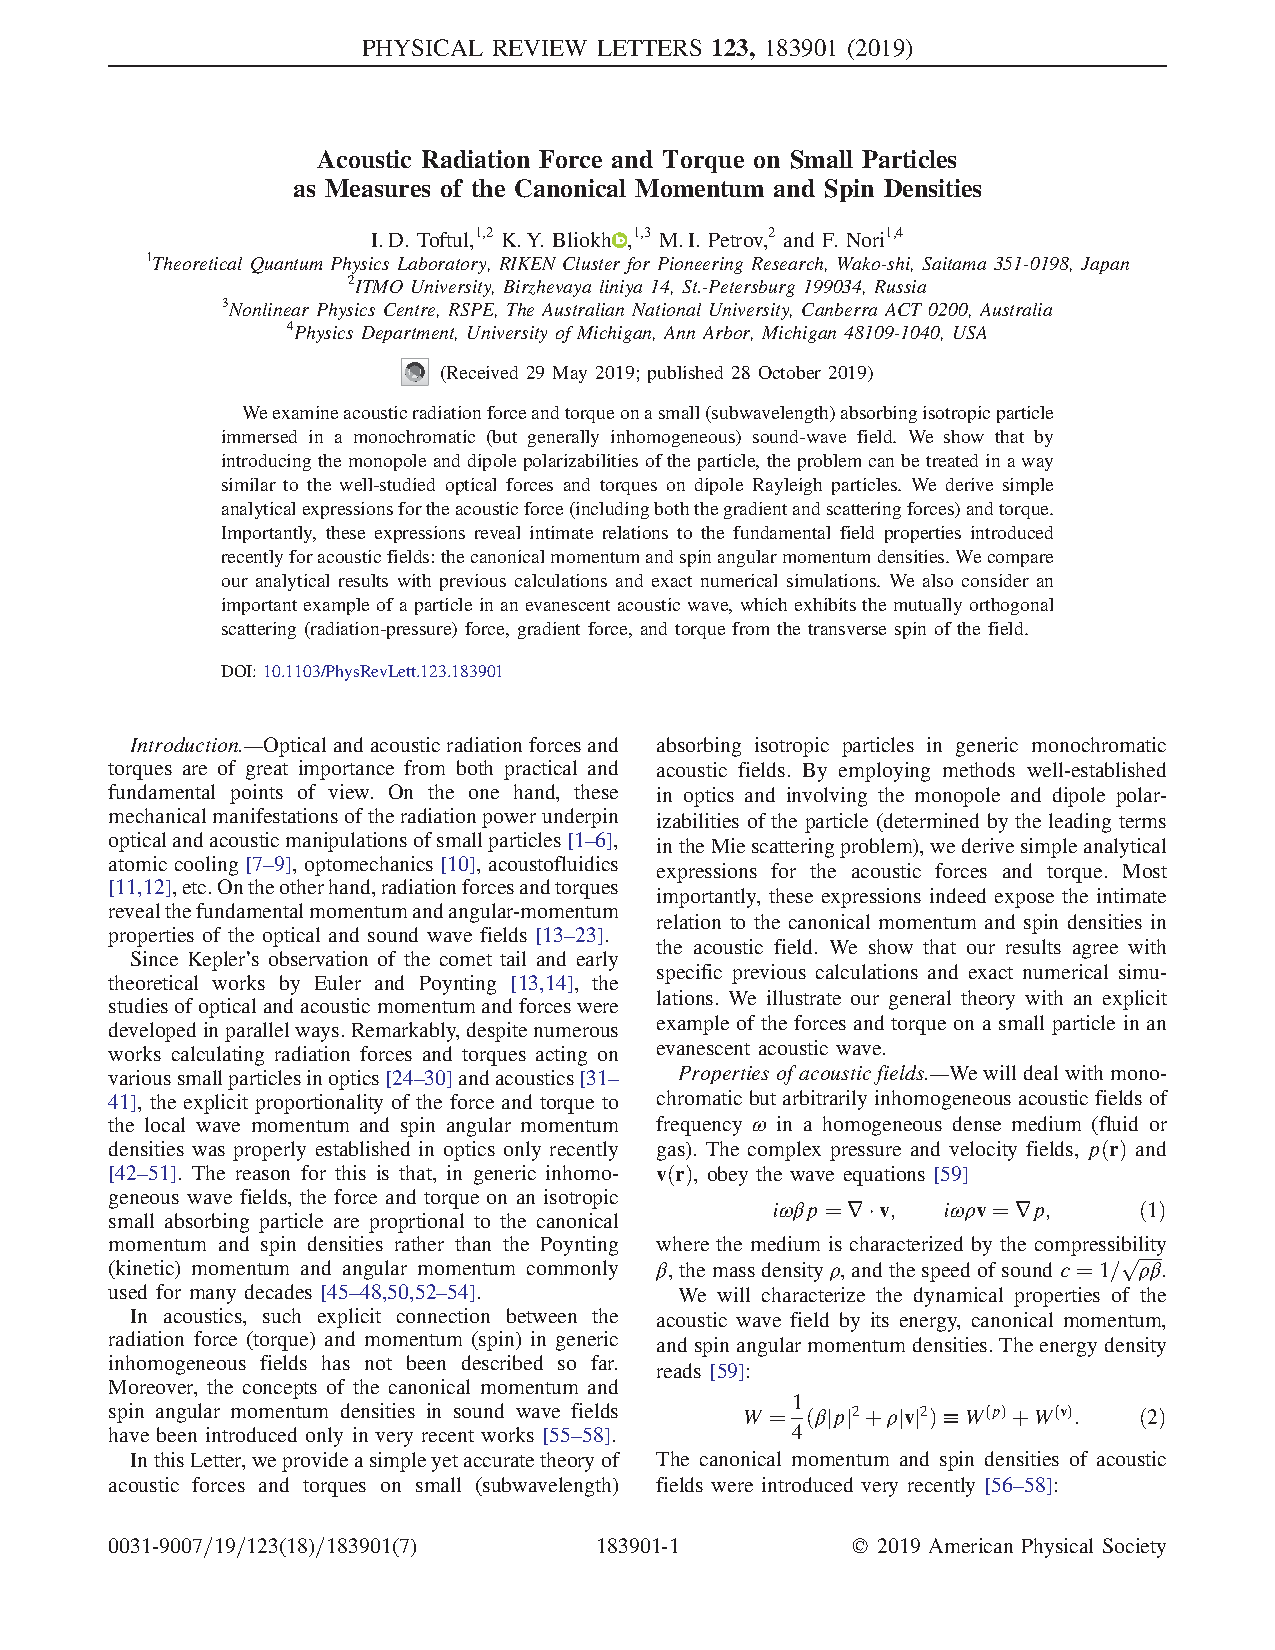
\includepdf[
%     pages={-},  % include all pages
%     pagecommand={},  % to include global numbering
%     scale=0.85,  % to leave space for the global page numbers
%     frame,  % adds a frame, optional
% ]{biblio/MyPublications/2019_PRL_acoustic.pdf}

        % Приложения, тут же свои публикации

\setcounter{totalappendix}{\value{chapter}} % Подсчёт количества приложений


\end{document}
